\documentclass[twoside]{article}

% file's preambule


% connect packages
%%%%%%%%%%%%%%%%%%%%%%%%%%%%%%%%%%%%%%%%%%%%%%%%%%%%%%%%%%%%%%%%%%%%%%
\usepackage[T2A]{fontenc}                   %!? закрепляет внутреннюю кодировку LaTeX
\usepackage[utf8]{inputenc}                 %!  закрепляет кодировку utf8
\usepackage[english,russian]{babel}         %!  подключает русский и английский
\usepackage{amsmath}                        %!  |
\usepackage{amssymb,textcomp, esvect,esint} %!  |важно для формул 
\usepackage[margin=2cm]{geometry}           %!  фиксирует оступ на 2cm
\usepackage{amsfonts}                       %!  математические шрифты
\usepackage{amsthm}                         %!  newtheorem и их сквозная нумерация
\usepackage{graphicx}                       %?  графическое изменение текста
\usepackage{indentfirst}                    %   добавить indent перед первым параграфом
\usepackage{xcolor}                         %   добавляет цвета
\usepackage{enumitem}                       %!  задание макета перечня.
\usepackage[unicode, pdftex]{hyperref}      %!  оглавление для панели навигации по PDF-документу + гиперссылки
\usepackage{booktabs}                       %!  добавляет книжные линии в таблицы
\usepackage{hypcap}                         %?  адресация на картинку, а не на подпись к ней
\usepackage{abraces}                        %?  фигурные скобки сверху или снизу текста
\usepackage{caption}                        %-  позволяет корректировать caption 
\usepackage{multirow}                       %   объединение ячеек в таблицах
\usepackage{pifont}                         %!  нужен для крестика
\usepackage{cancel}                         %!  аутентичное перечеркивание текста
\usepackage{ulem}                           %!  перечеркивание текста
\usepackage{tikz}                           %!  высокоуровневые рисунки (кружочек)
\usepackage{titling}                        %-  автоматическое заглавие 
\usepackage{blindtext}                      %-  слепой текст
\usepackage{fancyhdr}                       %   добавить верхний и нижний колонтитул

\usepackage{import}
\usepackage{xifthen}
\usepackage{pdfpages}
\usepackage{transparent}

\usepackage{mathrsfs}  
%%%%%%%%%%%%%%%%%%%%%%%%%%%%%%%%%%%%%%%%%%%%%%%%%%%%%%%%%%%%%%%%%%%%%%

%%%%%%%%%%%%%%%%%%%%%%% ИНТЕГРАЛЫ %%%%%%%%%%%%%%%%%%%%%%%%%%%%%%%%%%%%
\makeatletter
\def\upintkern@{\mkern-7mu\mathchoice{\mkern-3.5mu}{}{}{}}
\def\upintdots@{\mathchoice{\mkern-4mu\@cdots\mkern-4mu}%
 {{\cdotp}\mkern1.5mu{\cdotp}\mkern1.5mu{\cdotp}}%
 {{\cdotp}\mkern1mu{\cdotp}\mkern1mu{\cdotp}}%
 {{\cdotp}\mkern1mu{\cdotp}\mkern1mu{\cdotp}}}
\newcommand{\upiint}{\DOTSI\protect\UpMultiIntegral{2}}
\newcommand{\upiiint}{\DOTSI\protect\UpMultiIntegral{3}}
\newcommand{\upiiiint}{\DOTSI\protect\UpMultiIntegral{4}}
\newcommand{\upidotsint}{\DOTSI\protect\UpMultiIntegral{0}}
\newcommand{\UpMultiIntegral}[1]{%
  \edef\ints@c{\noexpand\upintop
    \ifnum#1=\z@\noexpand\upintdots@\else\noexpand\upintkern@\fi
    \ifnum#1>\tw@\noexpand\upintop\noexpand\upintkern@\fi
    \ifnum#1>\thr@@\noexpand\upintop\noexpand\upintkern@\fi
    \noexpand\upintop
    \noexpand\ilimits@
  }%
  \futurelet\@let@token\ints@a
}
\makeatother

\DeclareFontFamily{OMX}{mdbch}{}
\DeclareFontShape{OMX}{mdbch}{m}{n}{ <->s * [0.8]  mdbchr7v }{}
\DeclareFontShape{OMX}{mdbch}{b}{n}{ <->s * [0.8]  mdbchb7v }{}
\DeclareFontShape{OMX}{mdbch}{bx}{n}{<->ssub * mdbch/b/n}{}

\DeclareSymbolFont{uplargesymbols}{OMX}{mdbch}{m}{n}
\SetSymbolFont{uplargesymbols}{bold}{OMX}{mdbch}{b}{n}
\DeclareMathSymbol{\upintop}{\mathop}{uplargesymbols}{82}
\DeclareMathSymbol{\upointop}{\mathop}{uplargesymbols}{"49}

\DeclareFontEncoding{MDB}{}{}
\DeclareFontFamily{MDB}{mdbch}{}
\DeclareFontShape{MDB}{mdbch}{m}{n}{ <->s * [0.8]  mdbchrmb }{}
\DeclareFontShape{MDB}{mdbch}{b}{n}{ <->s * [0.8]  mdbchbmb }{}
\DeclareFontShape{MDB}{mdbch}{bx}{n}{<->ssub * mdbch/b/n}{}
\DeclareFontSubstitution{MDB}{cmr}{m}{n}
\DeclareSymbolFont{mathdesignB}{MDB}{mdbch}{m}{n}%
\SetSymbolFont{mathdesignB}{bold}{MDB}{mdbch}{b}{n}%
\DeclareMathSymbol{\upintclockwise}{\mathop}{mathdesignB}{128}
\DeclareMathSymbol{\upointclockwise}{\mathop}{mathdesignB}{130}
\DeclareMathSymbol{\upointctrclockwise}{\mathop}{mathdesignB}{132}
\DeclareMathSymbol{\upoiint}{\mathop}{mathdesignB}{134}
\DeclareMathSymbol{\upoiiint}{\mathop}{mathdesignB}{136}

\makeatletter
\newcommand{\upint}{\DOTSI\upintop\ilimits@}
\newcommand{\upoint}{\DOTSI\upointop\ilimits@}
\makeatother

%%%%%%%%%%%%%%%%%%%%%%%%%%%%%%%%%%%%%%%%%%%%%%%%%%%%%%%%%%%%%%%%%%%%%%



% add (renew) commands
%%%%%%%%%%%%%%%%%%%%%%%%%%%%%%%%%%%%%%%%%%%%%%%%%%%%%%%%%%%%%%%%%%%%%%
\renewcommand{\Im}{\mathop{\mathrm{Im}}\nolimits}
\renewcommand{\Re}{\mathop{\mathrm{Re}}\nolimits}
\renewcommand{\div}{\mathop{\mathrm{div}}\nolimits}
\renewcommand{\d}{\, d}
\renewcommand{\leq}{\leqslant}
\renewcommand{\geq}{\geqslant}

\newcommand{\vc}[1]{\mbox{\boldmath $#1$}}
\newcommand{\T}{^{\text{T}}}

\newcommand{\grad}{\mathop{\mathrm{grad}}\nolimits}
\newcommand{\rot}{\mathop{\mathrm{rot}}\nolimits}
\newcommand{\diag}{\mathop{\mathrm{diag}}\nolimits}
\newcommand{\Ker}{\mathop{\mathrm{Ker}}\nolimits}
\newcommand{\Spec}{\mathop{\mathrm{Spec}}\nolimits}
\newcommand{\sign}{\mathop{\mathrm{sign}}\nolimits}
\newcommand{\tr}{\mathop{\mathrm{tr}}\nolimits}
\newcommand{\rg}{\mathop{\mathrm{rg}}\nolimits}

\newcommand{\const}{\text{const}}
\newcommand{\red}[1]{\textcolor{red}{#1}}
\newcommand{\xmark}{\ding{55}}

\renewcommand{\int}{\upint}
\renewcommand{\oint}{\upoint}
%%%%%%%%%%%%%%%%%%%%%%%%%%%%%%%%%%%%%%%%%%%%%%%%%%%%%%%%%%%%%%%%%%%%%%


% some tikz commands
%%%%%%%%%%%%%%%%%%%%%%%%%%%%%%%%%%%%%%%%%%%%%%%%%%%%%%%%%%%%%%%%%%%%%%
\makeatletter %%%%%%%%%%%%%%% КРУЖОЧЕК %%%%%%%%%%%%%%%%%%%%%%%%%%%%%%%
\newcommand*{\encircled}[1]{\relax\ifmmode\mathpalette
\@encircled@math{#1}\else\@encircled{#1}\fi}
\newcommand*{\@encircled@math}[2]{\@encircled{$\m@th#1#2$}}
\newcommand*{\@encircled}[1]{%
  \tikz[baseline,anchor=base]{\node[draw,circle,outer sep=0pt,
                                        inner sep=.2ex] {#1};}}
\makeatother

\usepackage{arydshln} %%%%%%%%%%%%%%% ЛИНИИ В МАТРИЧКЕ %%%%%%%%%%%%%%%
\makeatletter
  \renewcommand*\env@matrix[1][*\c@MaxMatrixCols c]{%
    \hskip -\arraycolsep
    \let\@ifnextchar\new@ifnextchar
  \array{#1}}
\makeatother
%%%%%%%%%%%%%%%%%%%%%%%%%%%%%%%%%%%%%%%%%%%%%%%%%%%%%%%%%%%%%%%%%%%%%%



\DeclareRobustCommand{\tmpsim}{ %%%%%%%%%%%%%% ~ < %%%%%%%%%%%%%%%%%%%
  \mathbin{\text{
      \raisebox{-1pt}{
            \hspace{-4.5pt} \rotatebox{-26}{\scalebox{0.8}[0.7]{$\sim$}}
        }
  }}
}
\def\lesim{{
    \setbox0\hbox{$\ <\ $}
    \rlap{\hbox to \wd0{\hss$\tmpsim$\hss}}\box0
}}
%%%%%%%%%%%%%%%%%%%%%%%%%%%%%%%%%%%%%%%%%%%%%%%%%%%%%%%%%%%%%%%%%%%%%%


% create environment
%%%%%%%%%%%%%%%%%%%%%%%%%%%%%%%%%%%%%%%%%%%%%%%%%%%%%%%%%%%%%%%%%%%%%%
\newtheorem{to_thr}{Thr}[section]
\newtheorem{to_suj}[to_thr]{Suj}
\newtheorem{to_lem}[to_thr]{Lem}
\newtheorem{to_law}[to_thr]{Law}
\newtheorem{to_com}[to_thr]{Com}
\newtheorem{to_con}[to_thr]{Con}
\theoremstyle{definition}
\newtheorem{to_def}[to_thr]{Def}

\newenvironment{description*}
{
    \begin{description}
        \setlength{\itemsep}{1pt}
        \setlength{\parskip}{1pt}
        }
    {\end{description}
}
%%%%%%%%%%%%%%%%%%%%%%%%%%%%%%%%%%%%%%%%%%%%%%%%%%%%%%%%%%%%%%%%%%%%%%

\newcommand{\incfig}[1]{%
    % \def\svgwidth{\columnwidth}
    \import{./figures/}{#1.pdf_tex}
}

% add some colors
%%%%%%%%%%%%%%%%%%%%%%%%%%%%%%%%%%%%%%%%%%%%%%%%%%%%%%%%%%%%%%%%%%%%%%
\definecolor{grey}{HTML}{666666}
\definecolor{linkcolor}{HTML}{0000CC}
\definecolor{urlcolor}{HTML}{006600}
\hypersetup{
    pdfstartview=FitH,  
    linkcolor=linkcolor,
    urlcolor=urlcolor, 
    colorlinks=true,
    citecolor=blue}
%%%%%%%%%%%%%%%%%%%%%%%%%%%%%%%%%%%%%%%%%%%%%%%%%%%%%%%%%%%%%%%%%%%%%%


% add page header
%%%%%%%%%%%%%%%%%%%%%%%%%%%%%%%%%%%%%%%%%%%%%%%%%%%%%%%%%%%%%%%%%%%%%%
\pagestyle{fancy}
\fancyhf{}
\fancyhead[RE,LO]{\textsc{Ф\raisebox{-1.5pt}{и}з\TeX}}
% \fancyhead[LE,RO]{ОбщеФиз}
\fancyhead[CO,CE]{\leftmark}
\fancyfoot[LE,RO]{\textcolor{grey}{\texttt{\thepage}}}
%%%%%%%%%%%%%%%%%%%%%%%%%%%%%%%%%%%%%%%%%%%%%%%%%%%%%%%%%%%%%%%%%%%%%%


\begin{document}

% set skip of equation length 

\setlength{\abovedisplayskip}{3pt}
\setlength{\abovedisplayshortskip}{3pt}
\setlength{\belowdisplayskip}{3pt}
\setlength{\belowdisplayshortskip}{3pt}

% \numberwithin{equation}{section}

% input files


\section*{Articles used}

\begin{enumerate}[label = \Roman*.]
	\item <<Dynamics of Gliding Arc Climbing
in a Unipolar Jacob’s Ladder>> by K. I. Almazov et al. 22 January 2020;

	\item <<Physical study of a gliding arc discharge>> by F. Richard et al. 20 November 1995;

	\item <<Prospects of airflow control by a gliding arc in a static magnetic field>> by N Balcon et al. 28 August 2008;

	\item <<Numerical Calculations of the Properties of Axially Symmetric Arc Columns>> by A.Wells March 1967.
\end{enumerate}
% %%%%%%%%%%%%%%%%%%%%%%%%%%%%%%%%%%%%%%%%%%%%%%%%%%%%%%%%%%%%%%%%%%%%%%%%%%%%
% \section{Principal variables and constants}
% %%%%%%%%%%%%%%%%%%%%%%%%%%%%%%%%%%%%%%%%%%%%%%%%%%%%%%%%%%%%%%%%%%%%%%%%%%%%


% The heat flux potential (потенциал теплового потока) -- 

% The Prandtl and turbulent Prandtl numbers -- 

% The eddy diffusivity for momentum (вихревой коэффициент диффузии для импульса) -- 

% The specific enthalpy (удельная энтальпия) --



%%%%%%%%%%%%%%%%%%%%%%%%%%%%%%%%%%%%%%%%%%%%%%%%%%%%%%%%%%%%%%%%%%%%%%%%%%%%
\section{Principal equations (I article)}
%%%%%%%%%%%%%%%%%%%%%%%%%%%%%%%%%%%%%%%%%%%%%%%%%%%%%%%%%%%%%%%%%%%%%%%%%%%%


\subsection{Hand waving}

I would like to write the energy equation: the rate of change of energy per unit volume. To do this, we look at heat exchange with the environment and at movement in an electromagnetic potential field.

In fact $E^2\sigma$ -- specific energy density per unit time. We also have some heat exchange with the environment.
The heat flux potential can be defined by
\begin{equation}
    S = \int_0^T \varkappa \d T,
\end{equation}
So we characterize it as $\div \grad S = \nabla^2 S$, --  specific heat exchange. Then
\begin{equation*}
    P = \sigma E^2 + \div \grad S.
\end{equation*}
We expect to see something like that.

\subsection{According to the article}


Taking into consideration only a small part of the arc, we
define a set of axes $(r,x)$ in cylindrical coordinates.
\textbf{The energy equation} for a \textbf{steady arc} is
\begin{equation}
    \rho U \frac{\partial h}{\partial x} + \rho V \frac{\partial h}{\partial r} 
    =
    \frac{1}{r} \frac{\partial }{\partial r} 
    \left[
        r \left(\frac{\mu}{P_r} + \frac{\rho \varepsilon_m}{P_{rt}} \right) 
        \frac{\partial h}{\partial r} 
    \right] + 
    \sigma E^2,
\end{equation}
and \textbf{the continuity equation} by
\begin{equation} % вроде готовы в это верить. 
    \div \vc{j}_m = \frac{1}{r} \frac{\partial }{\partial r} (r \rho V) + \frac{\partial }{\partial x} (\rho U) = 0,
\end{equation}
where $\rho$ is the density, $U$ the axial velocity, $V$ the radial velocity, $h$ the specific enthalpy, $\mu$ the viscosity, $\varepsilon_m$ the eddy diffusivity for momentum, $P_\text{t}$ and $P_\text{rt}$ the Prandtl and turbulent Prandtl numbers, respectively, $\sigma$ the electrical conductivity, and $E$ the voltage gradient.

The heat flux potential can be defined by
\begin{equation*}
    S_{(T)} = \int_0^T \varkappa_{(T)} \d T,
\end{equation*}
so that the \textbf{molecular diffusion term}
\begin{equation*}
    \frac{1}{r} \frac{\partial }{\partial r} \left[
        r \left(\frac{\mu}{P_r} \right) \frac{\partial h}{\partial r} 
    \right] \equiv \nabla^2 S
\end{equation*}
in the energy equation can be replaced.


%%%%%%%%%%%%%%%%%%%%%%%%%%%%%%%%%%%%%%%%%%%%%%%%%%%%%%%%%%%%%%%%%%%%%%%%%%%%
\subsection{Assumptions}
%%%%%%%%%%%%%%%%%%%%%%%%%%%%%%%%%%%%%%%%%%%%%%%%%%%%%%%%%%%%%%%%%%%%%%%%%%%%


To describe the arc, we use a simplified model in which
rough assumptions are made. These assumptions were used 
by Maecker and Frind to describe cylindrical arc behavior. 
\begin{enumerate*}
    \item Flow is axially symmetrical.
    \item Viscous dissipation and Lorentz forces can be neglected.
    \item  Radial pressure gradient is negligible compared to the
        static pressure.
    \item  Radiation is neglected.
    \item  Principal transfer of energy is produced by conduction
        and convection.
\end{enumerate*}


We consider two arc regions separately -- 
\textbf{the plasma core}, 
also called plasma string, 
and 
\textbf{the outer flame} or weak ionized ring.




%%%%%%%%%%%%%%%%%%%%%%%%%%%%%%%%%%%%%%%%%%%%%%%%%%%%%%%%%%%%%%%%%%%%%%%%%%%%
\subsection{The plasma string model}
%%%%%%%%%%%%%%%%%%%%%%%%%%%%%%%%%%%%%%%%%%%%%%%%%%%%%%%%%%%%%%%%%%%%%%%%%%%%

Based on experimental results, although the arc is moving, the plasma channel can be considered to be \textbf{in a steady state with a constant radius}. Physical properties along the center line of the plasma string are assumed to be the same at
every point on the line. As a result of the longitudinal convection affecting the arc, the form is assumed to be cylindrical.

Let us consider a small part of the plasma string which is assumed to be identical to any other section of the plasma arc.

The emission of light being the same all along the string,
we assume
\begin{equation}
    \frac{\partial h}{\partial x} = 0.
\end{equation}
Turbulent effects and radial convection can be neglected for heat exchanges
\begin{equation}
    V \frac{\partial h}{\partial r} = 0.
\end{equation}
The energy equation is rewritten
\begin{equation}
    0   =
    \frac{1}{r} \frac{\partial }{\partial r} 
    \bigg[
        r \bigg(\frac{\mu}{P_r} + 
        \underbrace{\frac{\rho \varepsilon_m}{P_{rt}}}_{0?}
        \bigg) 
        \frac{\partial h}{\partial r} 
    \bigg] + \sigma E^2,
\end{equation}
rewriting in a different form,
\begin{equation}
    \nabla^2 S + \sigma E^2 = 0,
\end{equation}
which corresponds to the well known (авторами статьи) \textbf{Elenbaas–Heller equation}.


%%%%%%%%%%%%%%%%%%%%%%%%%%%%%%%%%%%%%%%%%%%%%%%%%%%%%%%%%%%%%%%%%%%%%%%%%%%%
\subsection{The arc core-outer flame transition}
%%%%%%%%%%%%%%%%%%%%%%%%%%%%%%%%%%%%%%%%%%%%%%%%%%%%%%%%%%%%%%%%%%%%%%%%%%%%

At the boundary of the arc core and the outer flame, the temperature profile in the plasma string is assumed to be invariable with a constant conducting radius $r_c$.


Convection is, therefore, the main cause of plasma string  cooling. It constricts the arc as the difference in velocity between arc–core and the surrounding region increases. The constant plasma string radius is evidence of an equivalent
constant convection effect expressed in terms of an axially symmetrical convection flow.

The convection term does not appear in the energy balance equation of the plasma string, but is implicitly taken into account in the input value of the electric field and power per unit of length deduced from experiments. 

In the conductive inner part of the discharge, the electrical conductivity is given as a linear function of heat flux potential
\begin{equation}
    \sigma = \beta (S - S_{\text{c}}),
\end{equation}
where $S_C$ is the heat flux potential for $\sigma=0$ correspondings to the conduction radius $r_c$.

 The conduction radius is 
\begin{equation}
    \vc{r}_c \sim \frac{1}{\sqrt{\beta} E} .
\end{equation}
The power per unit of discharge length $w$ is related to $S_0$ which corresponds to the axis heat flux potential ($r=0$), on which the temperature is $T_0$, according to the following equation:
\begin{equation*}
    S_0 = \frac{w}{2\pi} + S_c.
\end{equation*}


% \newpage
\section{Staged experiment (II articls)}


Devices with a gliding arc are classified according
to power supply regime as <<\textbf{bipolar}>> and \textbf{unipolar}>>.
In the bipolar regime of power supply, sign-alternating 
sinusoidal voltage is applied to two electrodes of a
device.

In this experiment and ours, we work with a Flyback transformer, so that the signal is rectified in the unipolar case.

\begin{figure}[h]
    \centering
    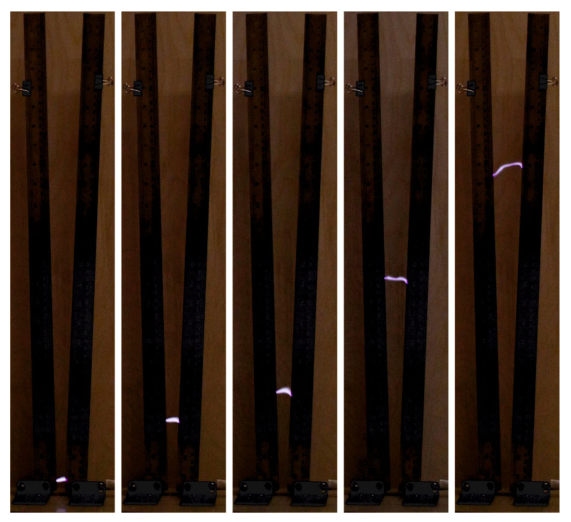
\includegraphics[width=0.3\textwidth]{figures/1.png}
    \caption{Experiment for Article II.}
\end{figure}

It was founded, that it moves with a constant velocity on most of the path. Also, the the dependence of the arc rise speed on the angle between the electrodes was investigated.


\section{Staged experiment (III articls)}


A slightly more meaningful experiment was set up in the next article, it has yet to be analyzed.

\begin{figure}[h]
    \centering
    \includegraphics[width=0.4\textwidth]{figures/2.png}
    %\caption{}
    %\label{fig:}
\end{figure}





% % document's head
% \phantom{42}

\begin{center}
    \LARGE \textsc{Заметки курса <<Электричество и магнетизм>>}
\end{center}

\hrule

\phantom{42}

\begin{flushright}
    \begin{tabular}{rr}
    % written by:
        \textbf{Автор}: 
        & Хоружий Кирилл \\
        &\\
    % date:
        \textbf{От}: &
        \textit{\today}\\
    \end{tabular}
\end{flushright}

\thispagestyle{empty}
\tableofcontents
% \newpage


% \input
% \input







\end{document} \begin{to_def}[Свертка функции] Свёртку ещё пишут как $h = f * g$.
	\begin{equation*}
		h(x) = \int_{\mathbb{R}^n} f (x - t)g(t)\d t =\int_{\mathbb{R}^n} f(t)g(x-t) \d t,
	\end{equation*}
	\label{def_svertka}
\end{to_def}

Свёртка также ассоциативна: $f *(g*h) = (f*g)*h$, для функций с конечным интегралом.
Чтобы интеграл существовал, можно заметить, что если одна из функций ограничена, а другая имеет конечный интеграл, тогда и свёртка будет ограничена, кроме того:

\begin{to_thr}%[\ref{proof_6.18}]
	Если $f$ и $g$ имеют конечный интегралы, \textbf{то} $h = f*g$ определена почти всюду и верно неравенс{}тво
	\begin{equation*}{}
		\int_{\mathbb{R}^n} |f * g| \d x < \int_{\mathbb{R}^n}|f| \d x \cdot \int_{\mathbb{R}^n}|g|\d x,
	\end{equation*}
	и равенство:
	\begin{equation*}
		\int_{\mathbb{R}^n} f * g \d x = \int_{\mathbb{R}^n} f \d x \cdot \int_{\mathbb{R}^n} g \d x.
	\end{equation*}
	\label{thr_6.18}
\end{to_thr}

\begin{to_lem}
	Если свёртка $g*f$ --- \textbf{ограничена}, где $g$ -- имеет конечный интеграл, а $f$ и $\partial_x f$ -- ограничены, \textbf{то} возможно \text{дифференцирование под знаком интеграла} (\ref{5.95}), и мы получаем:
	\begin{equation*}
		\frac{\partial (f*g)}{\partial x_i} = \int_{\mathbb{R}^n} \frac{\partial f(x-t)}{\partial x_i} g(t) \d t = \frac{\partial f}{\partial x_i} * g.
	\end{equation*}
	\label{lem_6.19}
\end{to_lem}
Возьмём $f \in C^\infty$ такую, что $\forall k f^{(k)} (0) = 0$. Из неё составим $\varphi\in C^\infty$ большую нуля на $(-1,1)$:
\begin{equation*}
	f(x) = \left\{
	\begin{aligned}
	    &0, &x\leq 0; \\
	    &e^{-1/x}, &x>0.
	\end{aligned}\right.
	\hspace*{1 cm} \varphi(x) = f(x+1) f(1-x).
\end{equation*}

\begin{to_lem}
	$\forall \varepsilon > 0 \; \exists$ бесконечно гладкая $\varphi_\varepsilon \colon \mathbb{R}^n \rightarrow \mathbb{R}^+$, $\varphi_\varepsilon(x) \neq 0 \; \forall x \in U_\varepsilon(0)$, \textbf{такая чтo} $\int_{\mathbb{R}^n} \varphi_\varepsilon(x) \d x = 1. $
	\label{lem_6.20}
\end{to_lem}

\begin{to_lem}
	$\forall \varepsilon > \delta > 0 \; \exists$
	бесконечно гладкая $\psi_{\varepsilon,\delta} \colon \mathbb{R}^n \rightarrow [0,1] $,
	$\psi_{\varepsilon,\delta}(x) \neq 0 \; \forall x \in U_\varepsilon(0)$ 
	и $\psi_{\varepsilon,\delta} (x) \neq 0 \; \forall x \in U_\delta(0)$.
\end{to_lem}Пусть $\varphi\colon \mathbb{R}^n \rightarrow \mathbb{R} $, неотрицательная $\varphi\in C^\infty $, $\varphi \neq 0$ при $|x| \leq 1$ и пусть $\int_{\mathbb{R}^n} \varphi(x) \d x = 1$.
Положим  $\varphi_k (x) = k^n \varphi(k x) $, у которых так же будут $\int = 1$ и которые $ \varphi_k \neq 0$ при $|x| \leq 1/k$.

\begin{to_thr}
	Для непрерывной $f \colon \mathbb{R}^n \rightarrow \mathbb{R} $ определим свёртки:
	\begin{equation*}
		f_k(x) = \int_{\mathbb{R}^n} f(x-t)\varphi_k \d t = \int_{\mathbb{R}^n} f(t) \varphi_k (x -t) \d t \hspace*{0.5 cm} \leadsto \hspace*{0.5 cm} f_k \in C^\infty, \; f_k \rightarrow f \text{ равномерно на компактах в } \mathbb{R}^n.
	\end{equation*}
	\label{thr_6.21}
\end{to_thr}

\begin{to_thr}
	Если $f$ имеет непр. производные до $m$-го порядка, то производные $f_k$ до $m$-го порядка равномерно сходятся на компактах к соответствующим $f'$.
	\label{thr_6.22}
\end{to_thr}

\begin{to_thr}
	Пусть $f\colon \mathbb{R}^n \rightarrow \mathbb{R}$ и $f \in \L_{c}$. Тогда свёртки $f*\varphi_k$ c функциями из теоремы \ref{thr_6.21} сколь угодно близко приближают $f$ в среднем.
	\label{thr_6.23}
\end{to_thr}% 6.1. Дифференцируемые отображения открытых подмножеств R n .
\begin{to_def} 
    Пусть $U \subset \mathbb{R}^n$ -- открытое множество. Отображение $f \colon U \to \mathbb{R}^m$ называется \textit{дифференцируемым} в точке $x_0 \in U$, если
    \begin{equation*}
        f(x) = f(x_0) + Df_{x_0} (x - x_0) + o(|x-x_0|), \hspace{0.5cm} x \to x_0,
    \end{equation*} 
    где $Df_{x_0} \colon \mathbb{R}^n \mapsto \mathbb{R}^m$ -- линейное отображение, называемое \textit{производной} $f$ в точке $x_0$.  
\end{to_def}

\begin{to_def} 
    Функция $f$ называется \textit{непрерывно дифференцируемой} на $U$, если оно  дифференцируемо в каждой точке и $Df_x$ непрерывно зависит от $x$.
\end{to_def}

\begin{to_thr}[Дифференицрование композиции]
     Если $f$ дифференцируемо в точке $x_0$, $g$ дифференцируемо в точке $y_0 = f(x_0)$, то композиция $g \circ f$ дифференцируема в точке $x_0$, и $D(g \circ f)_{x_0} = Dg_{y_0} \circ Df_{x_0}$.
\end{to_thr}


\begin{to_def} 
    Производная функции $f$ по направлению $v \in Rn$ в точке $x$ называется
    \begin{equation*}
         \frac{\partial f}{\partial v} = 
         \lim_{t \to 0}
         \left(\frac{f(x + t v) - f(x)}{t} \right)
     \end{equation*} 
\end{to_def}

\begin{to_lem} 
    Если функция дифференцируема в точке $x$, то в этой точке
    \begin{equation*}
         \frac{\partial f}{\partial v} = Df_x (v).
     \end{equation*} 
     В частности для функционалов, верно что $\partial f / \partial v = df_x (v)$. Более того, выбрав в качестве $v$ базисные векторы $e_i$, поймём что
     \begin{equation*}
         df = \frac{\partial f}{\partial x^i} x^i,
     \end{equation*}
     где $dx^i$ -- дифференциалы координатных функций, образующие двойственный базис.
\end{to_lem}

\begin{to_thr} 
    Если отображение $f \colon U \mapsto \mathbb{R}^m$ из открытого $U \subseteq \mathbb{R}^n$ задано в координатах, как $y_i = f_i(x_1, \ldots, x_n)$, для $i = 1,\ldots,m$ и функции $f_i$ имеют непрерывные частные производные на $U$, то $f$ непрерывно дифференцируемо на $U$. 
\end{to_thr}% 6.4. Непрерывно дифференцируемые отображения и криволинейные системы координат

\begin{to_def} 
    \textit{Криволинейная замена координат} --- бесконечно гладкое отображение $\varphi \colon U \mapsto  V$ такое, что $\varphi^{-1}$ определено и тоже бесконечно гладко. 
\end{to_def}

\begin{to_lem} 
    Пусть открытое множество $U \subset \mathbb{R}^n $ выпукло. Для непрерывно дифференцируемого отображения $\varphi \colon U \to \mathbb{R}^m $ найдётся непрерывное отображение $A \colon U \times U \mapsto  \mathcal L (\mathbb{R}^n, \mathbb{R}^m)$, такое что $\forall x', \ x'' \in U$ 
\begin{equation*}
     \varphi(x'') - \varphi(x') = A(x', x'')(x'' - x')
 \end{equation*} 
 и $A(x, x) = D \varphi_x$.  
\end{to_lem}

% \begin{to_lem} 
%     Для всякого линейного отображения $A \colon \mathbb{R}^n \mapsto \mathbb{R}^m$ найдётся число $\|A\|$ такое что для все $x \in \mathbb{R}^n$ $|Ax| \leq \|A\| \cdot |x|$. 
% \end{to_lem}

\begin{to_thr}[Теорема об обратном отображении]
     \textbf{Если} отображение $\varphi \colon U \mapsto \mathbb{R}^n$ непрерывно дифференцируемо в окрестности точки $x$ \textbf{и} его дифференциал $D\varphi_x$ являетсяя невырожденным линейным преобразованием, \textbf{то} это отображение взаимно однозначно отображает некоторую окрестность $V \ni x$ на окрестность $W \ni y$, где $y = \varphi(x)$. Обратное отображение $\varphi^{-1} \colon W \to V$ тоже непрерывно дифференцируемо. 
\end{to_thr}


\begin{to_def} 
    \textit{Криволинейной системой координат} в окрестности точки $p \in \mathbb{R}^n$ называется набор таких функций, которые явяются координатами гладкого отображения окрестности $p$ на некоторое открытое множество в $\mathbb{R}^n$ с гладким обратным\footnote{
        По теореме об обратном отображении для проверки системы преобразования достаточно проверить невырожденность $\left(
    \partial y_i / \partial x_j
    \right)$ в точке $p$, или линейную независимость $dy^i$ в точке $p$.
    } отображением.
\end{to_def}

\begin{to_thr}[Теорема о неявной функции]
\label{thr_6.32}
     Пусть функции $f_1, \ldots, f_k$ непрерывно дифференцируемы в окрестности $p \in \mathbb{R}^n$ и 
    \begin{equation*}
        \det \left(
            \frac{\partial f_i}{\partial x_j} 
        \right) \neq 0
    \end{equation*}
    в этой окрестности. Пусть $f_i(p) = y_i$, $i = 1, \ldots, k$. Тогда найдётся окрестность точки $p$ вида $U \times V$, $U \subset \mathbb{R}^k$, $V \subset \mathbb{R}^{n-k}$, такая что в этой окрестности множество решений системы уравнений
    \begin{equation*}
        \left\{\begin{aligned}
            f_1(x) &= y_1, \\
            &\ldots \\
            f_k(x) &= y_k,
        \end{aligned}\right.
    \end{equation*}
    совпадает с графиком непрерывно дифференцируемого отображения $\varphi \colon V \to U$, заданного в координатах как
    \begin{equation*}
        \left\{\begin{aligned}
            x_1 &= \varphi_1 (y_1, \ldots, y_k,\ x_{k+1}, \ldots, x_n),\\
            &\ldots\\
            x_k &= \varphi_k (y_1, \ldots, y_k,\ x_{k+1}, \ldots, x_n),
        \end{aligned}\right.
    \end{equation*}
    то есть отображения $\mathbb{R}^{n-k} \mapsto \mathbb{R}^k$.
\end{to_thr}

\begin{to_thr}[Теорема о расщеплении отображения на элементарные]
     Если отображение $\varphi$ непрерывно дифференцируемо в окрестности точки $p \in \mathbb{R}^n$ и имеет обратимый $D \varphi_x$, то его можно представить в виде композиции перестановки координат, отображений координат и элементарных отображений, непрерывно дифференцируемо и возрастающим образом меняющих только одну координату $y_i = \psi_i (x_1, \ldots, x_n)$.
\end{to_thr}

\begin{to_thr} 
    Теоремы об обратном отображении, о неявной функции и о расщеплении отображения дают отображения класса $C^k$ при $k \geq 1$, если исходные отображени были класса $C^k$. 
\end{to_thr}\begin{to_def}
	Точка $p$ называется локальным экстремумом функции $f$, если она является точкой экстремума (максимума или минимума) ограничения $f$ на некоторую окрестность $p$.
	\label{def_6.36}
\end{to_def}

\begin{to_thr}[Необходимое условие экстремума]
	\begin{equation*}
		\left\{\begin{aligned}
	    	&f \in C^1(U(p))\\
	    	&p \text{ --- def(\ref{def_6.36})}
		\end{aligned} \right.
		\hspace*{0.5 cm} \Rightarrow \hspace*{0.5 cm}
		\d f_p = 0.
	\end{equation*}
	\label{thr_6.37}
\end{to_thr}

\begin{to_lem}
	Если квадратичная форма $Q > 0$, \textbf{то} $\exists \varepsilon>0 \colon $ $Q(v) \geq \varepsilon|v|^2 \;(\forall v)$.
	\label{lem_6.38}
\end{to_lem}
\begin{to_thr}[Необходимые условия экстремума]
	\begin{equation*}
	\left\{\begin{aligned}
	    	&f \in C^2(U(p))\\
	    	&p \text{ --- def(\ref{def_6.36})}
		\end{aligned} \right.
		\hspace*{0.5 cm} \Rightarrow \hspace*{0.5 cm}
		\left[
		\begin{aligned}
			\d_2 f_p \geq 0 \text{ --- min}\\
			\d_2 f_p \leq 0	\text{ --- max}
		\end{aligned}\right.
\end{equation*}	
\end{to_thr}

\begin{to_thr}[Достаточные условия экстремума]
\begin{equation*}
	\left\{\begin{aligned}
	    	&f \in C^2(U(p))\\
	    	&p \text{ --- def(\ref{def_6.36})}\\
	    	&\d f_p = 0 \text{ и } \d_2 f_p >0 
		\end{aligned} \right.
	\hspace*{0.5 cm}  \Rightarrow \hspace*{0.5 cm}
	p \text{ --- точка строгого локального максимума}
	\label{thr_6.39}
\end{equation*}
\end{to_thr}\begin{to_def}
	Условный экстремум f --- экстремум ограничения $f$ на множество $S$, задаваемое системой $C^1$ уравнений $\varphi_1(x) = \ldots = \varphi_m(x) = 0$.

	Забегая вперёд, нам самом деле нам нужно: $\dim \langle \d \varphi_1, \ldots, \d \varphi_m\rangle = m$.
	\label{def_usl_ext}
\end{to_def}

\begin{to_thr}[Необходимые условия условного экстремума в терминах первых производных]
	 \begin{equation*}
	 \left\{
	 	\begin{aligned}
	 		&f, \varphi_1,\ldots,\varphi_m \in C^1(U(p))\\
	 		&\dim \langle \d \varphi_1, \ldots, \d \varphi_m\rangle = m\\
	 		&p \text{ --- def(\ref{def_usl_ext})}
	 	\end{aligned}\right.
	 	\hspace*{0.5 cm} \Rightarrow \hspace*{0.5 cm}
	 	\d f_p = \lambda_1 \d \varphi_{1,p} + \ldots + \lambda_m \d \varphi_{m,p}.
	 \end{equation*}
	 \label{thr_6.41}
\end{to_thr}
Удобно положить: $L(x) = f(x) - \lambda_1 \varphi_1(x) - \ldots - \lambda_m \varphi_m(x)$. Это называется \textit{функцией Лагранжа},а $\lambda_{i}$ --- \textit{множители Лагранжа}.

\begin{to_thr}[Необходимые условия условного экстремума]
	\begin{equation*}
	 \left\{
	 	\begin{aligned}
	 		&f, \varphi_1,\ldots,\varphi_m \in C^2(U(p))\\
	 		&\dim \langle \d \varphi_1, \ldots, \d \varphi_m\rangle = m\\
	 		&p \text{ --- def(\ref{def_usl_ext})}\\
	 		&\vc{v}\colon \d \varphi_{1,p}(\vc{v}) = \ldots = \d \varphi_{m,p}(\vc{v}) = 0
	 	\end{aligned}\right.
	 	\hspace*{0.5 cm} \Rightarrow \hspace*{0.5 cm}
	 	\left\{
	 	\begin{aligned}
	 		&\d L_p = 0\\
	 		&\left[
	 		\begin{aligned}
	 			&\d_2 L_p \geq 0 (\text{для минимума})\\
	 			&\d_2 L_p \leq 0 (\text{для максимума})
	 		\end{aligned}\right.
	 	\end{aligned}\right.
	 \end{equation*}
	 \label{thr_6.42}
\end{to_thr}

\begin{to_thr}[Достаточные условия условного экстремума]
	\begin{equation*}
		\left\{
		\begin{aligned}
	 		&f, \varphi_1,\ldots,\varphi_m \in C^2(U(p))\\
	 		&\dim \langle \d \varphi_1, \ldots, \d \varphi_m\rangle = m\\
	 		&\d L_p = 0\\
	 		&\varphi_1(p) = \ldots = \varphi_m(p) = 0\\
	 		&\vc{v}(\neq 0) \colon \d \varphi_{1,p}(\vc{v}) = \ldots = \d \varphi_{m,p}(\vc{v}) = 0\\
	 		&\d_2 L(\vc{v}) > 0 \text{ или } \d_2 L(\vc{v}) < 0
	 	\end{aligned}\right.
	 	\hspace*{0.5 cm} \Rightarrow \hspace*{0.5 cm}
	 	f \text{ имеет строгий условный экстремум в } p.
	\end{equation*}
	\label{thr_6.43}
\end{to_thr}

% 6.6. Векторы и векторные поля

\begin{to_lem} 
    \label{lem_6.44}
    Всякую гладкую функцию, определенную в некоторой окрестности $x_0 \in \mathbb{R}^n$, в возможно меньшей окрестности $x_0$, можно представить в виде
    \begin{equation*}
         f(x) = f(x_0) + \sum_{k=1}^n \partial_k f|_{x_0}
         \
         (x^k  - x_0^k) , 
     \end{equation*} 
     с гладкими $\partial_k f$.
\end{to_lem}

% Начнём наше удивительное приключение в определение вектора. Для всякого $v \in \mathbb{R}^n$ мы можем определеить производную по направлению
% \begin{equation*}
%     \frac{\partial f}{\partial v}  = \lim_{t \to 0} 
%     \left(
%         \frac{f(p+tv)-f(p)}{t} 
%     \right),
%     \hspace{0.5cm} 
%     \frac{\partial (fg)}{\partial v} = \frac{\partial f}{\partial v} g + f \frac{\partial g}{\partial v}.
% \end{equation*}
% Проблема -- $p + tv$ определено не инвариантно. Решение -- определим вектор, как \textit{дифференцирование алгебры гладких функций в точке}, удовлетворяющее формуле Лейбница.

\begin{to_def} 
    Определим \textit{касательный вектор} в точке $p \in U$ открытого множества $U \subseteq \mathbb{R}^n$ как $\mathbb{R}$-линейное отоборражение $X \colon C^{\infty}(U) \mapsto \mathbb{R}$, удовлетворяющее 
    \begin{equation*}
        X(fg) = X(f) g(p) + f(p) X(g).
    \end{equation*}
    \textit{Касательное пространство} $T_p U$ к $U$ в точке $p$ состоит из всех касательных векторов в точке $p$.
\end{to_def}

\begin{to_lem} 
    Если $X$ -- касательный вектор в точке $p \in U$, то для любой окресности $V \ni p$, $V \subseteq U$, выражение $X(f)$ может зависеть только от значений $f$ в $V$, а не на всём $U$. 
\end{to_lem}

В силу предыдущих лем мы можем перейти в окрестность, где $f$ представима в виде \eqref{lem_6.44}, тогда
\begin{equation*}
    X(f) = X(f(p)) + \sum_{i=1}^n X(x_i) \partial_i f|_p + \sum_{i=1}^n x_i(p) X(\partial_i f|_p) = 
    \sum_{i=1}^n X(x_i) \ \partial_i f|_p.
\end{equation*}
Числа $X_i = X(x_i)$ называются координатами касательного вектора в данной криволинейной системе координат, тогда весь вектор в точке $p$ записывается, как $X = X^i \partial_i$.

\begin{to_def} 
    \textit{Векторным полем} на открытом множестве $U \subseteq \mathbb{R}^n$ называется выбор касательного вектора $X(p) \in T_p U$ для каждой точки $p \in U$, гладко\footnote{
        Гладкая зависимость понимается в смысле гладкой зависимости координат векторного поля $X_i(p)$ в точке $p$.
    } зависящий от $p$.  
\end{to_def}


\begin{to_lem} 
    Для открытого $U \subseteq \mathbb{R}^n$ всякое $\mathbb{R}$-линейное отображение $X \colon C^{\infty} \mapsto C^{\infty}(U)$, удовлетворяющее правилу Лейбница $X(fg) = X(f) g + f x(g)$ задаётся векторным полем на $U$. 
\end{to_lem}



\begin{to_def} 
    Пусть есть вектор $X \in T_pU,$ $q = \varphi(p)$, тогда \textit{прямой\footnote{
        Производную отображения $\varphi$ в точке $p$ можно определить как $\varphi_*\colon T_p U \mapsto  T_q V$ при $q = \varphi(p)$. Иначе можем обозначать, как $F \varphi_p$.
    } образ вектора} $\varphi_*(X)$ определяется по формуле
    \begin{equation*}
        \varphi_* (X) f = X(f \circ \varphi),
        \hspace{1cm}\Rightarrow\  \left(\varphi_*X\right)^i = \frac{\partial \varphi^i}{\partial x^j} X^j 
        \hspace{0.25cm} \Leftrightarrow \hspace{0.25cm} 
        \text{\red{переписать в матричном виде}}
        .
    \end{equation*}
\end{to_def}

\begin{to_def} 
    Отображение $\varphi \colon U \mapsto  V$ задаёт \textit{гомоморфизм алшебр} (операция, сохраняющая умножение, сложение, и переводящая $\const$ в $\const$): 
    $\varphi^* \colon C^{\infty}(V) \mapsto C^{\infty}(U)$ по формуле
    \begin{equation*}
        \varphi^* (f) = f \circ \varphi.
    \end{equation*}
    вектор даёт дифференцирование алгебры $X \colon C^{\infty}(U) \mapsto \mathbb{R}$, и тогда $\varphi_* X = X \circ \varphi^*$ тоже дифференцирование алгебры. 
\end{to_def}

\begin{to_def} 
    \textit{Дифференциальная 1-форма} -- это ковекторное поле. Иначе, элемент двойственного пространства $(T_p U)^* \equiv T_p^* U$, линейная форма на касательнм пространстве, гладко зависящая от $p$. 
    \textit{Дифференциал} функции $f$ от векторного поля $X$ это $df (X) \overset{\mathrm{def}}{=} X f$.
\end{to_def}

Дифференциалы $dx_1, \ldots, dx_n$ дают базис $T_p^* U$, двойственный к $\partial_1, \ldots, \partial_n$, в смысле $dx^i \partial_j = \delta_j^i$. По этому базису можно разложить любую форму в точке, а применяя это $\forall p \in U \subseteq \mathbb{R}^n$ видим, что $\omega^1 = \alpha_i dx^i$.


При замене координат компоненты $\omega^1$ преобразуются как дифференциалы функции, то есть 
\begin{equation*}
    \alpha = \alpha_j dx^j = \tilde \alpha_i dy^i = 
    \underbrace{\tilde \alpha_i \partial_j y^i }_{\alpha_j}
    dx^j, \hspace{0.5cm} \Rightarrow \hspace{0.5cm} 
    \alpha_j = \tilde \alpha_i \partial_j y^i
    \hspace{0.25cm} \Leftrightarrow \hspace{0.25cm} 
    \text{\red{переписать в матричном виде}}.
\end{equation*}



% Дописать что происходит при замене базиса

% \red{Далее некоторые рассуждения из НМУ}. Заметим, что $\frac{\partial }{\partial x^1}, \ldots, \frac{\partial }{\partial x^n}$ -- базис в каждой точке. Рассмотрим теперь $f = x^i$ и $X = \frac{\partial }{\partial x^j} $, тогда
% \begin{equation}
%     d x^i \left(\frac{\partial }{\partial x^j} \right)
%     =
%     \frac{\partial x^i}{\partial x^j} = \delta^i_j.
% \end{equation}
% Из этого следует, что $dx_1,\ldots,dx_n$ -- двойственный к $\frac{\partial }{\partial x^1}, \ldots, \frac{\partial }{\partial x^n}$ базис в $V^*$.
% Тогда в этом базисе
% $$
%     d f = \omega_i \d x^i.
% $$
% Заметим, что
% $$
% \underbrace{\omega_i \d x^i }_{df}
%     \left(
%         \frac{\partial }{\partial x^j} 
%     \right) = \omega_i \delta^i_j = \omega_j,
%     \hspace{0.5cm} \Rightarrow \hspace{0.5cm} 
%     \omega_j = df \left(\frac{\partial }{\partial x^j} \right) =
%     \frac{\partial f}{\partial x^j}.
% $$
% Тогда
% \begin{equation}
%     df = \frac{\partial f}{\partial x^i} \d x^i.
% \end{equation}
% Получается ковектор $df$ расписывается по базису
% $dx^i$
%  двойственного пространства с координатами $\partial f / \partial x^i$.

% А для общей 1-формы
% $$
%     \omega = \omega_i \d x^i,
% $$
% где $\omega_1, \ldots, \omega_n$ -- координаты $\omega$ в локальной системе координат.

% \begin{to_def} 
%     $\omega$  гладкая, если $\forall X$, где $X$ -- гладкое поле, верно, что
%     $\omega(X)$ -- гладкая функция.
% \end{to_def}

% \begin{to_lem} 
%     $\omega = \omega_i \d x^i$  -- гладкая $\Leftrightarrow$ $\omega_i$ -- гладкая форма $\forall i$.
% \end{to_lem}

% \red{Конец рассуждений из НМУ}.\begin{to_def} 
    Определим \textit{дифференциальную форму степени} $k$ на открытом $U \subseteq \mathbb{R}^n$ как кососимметричное отображение наборов из $k$ гладких векторных полей $X_1, \ldots, X_k$ на $U$ в $C^{\infty}(U)$, линейное по каждому аргументу и относительно умножения на бесконечно гладкие функции.
\end{to_def}

\begin{to_lem} 
    Значение выражения $\alpha(X_1, \ldots, X_k)$ в точке $p$ зависит только от значений векторных полей $X_i$ в точке $p$.     
\end{to_lem}

Пространство диф-форм степени $k$ на $U \subseteq \mathbb{R}^n$ обозначим $\Omega^k(U)$. Интересно, что $\Omega^n(U)$ в фиксированной системе координат выглядит как $C^{\infty}(U)$, но при замене координат ведёт себя иначе.

% Для $ \forall f \in C^{\infty}(U)$ её дифференциал, как отображение $U \mapsto \mathbb{R}$ можно считать формой первой степени $df(X) = X(f)$. 


\red{Свойства диф-форм?}




\begin{to_def} 
    \textit{Внешнее умножение} $\Omega^k(U) \times \Omega^l (U) \mapsto \Omega^{k+l} (U)$, можно определить как $\alpha \wedge \beta = \text{Alt}\, (\alpha \otimes \beta)$, при чём $(dx_1 \wedge \ldots \wedge dx_k)(\partial_1, \ldots, \partial_k) = 1$.
\end{to_def}

\red{Здесь можно написать про операцию альтернирования.}\begin{to_lem} 
    На гладких диф-формах на $U$ существует единсвтенный $\mathbb{R}$-линейный оператор $\delta \colon \Omega^k (U) \mapsto \Omega^{k+1} (U)$, удовлетворяющий условиям: 
    1) $d(f) = df$;
    2) $d^2 = 0$;
    3) $d(\alpha \wedge \beta) = d \alpha \wedge \beta + (-1)^{\deg \alpha} \alpha \wedge d \beta$ (а-ля правило Лейбница).
    Более того, операция $d$ определена инвариантно.
\end{to_lem}

\begin{to_def}[Обратный образ] 
    Для всякого гладкого отображения $\varphi \colon U \mapsto V$ между открытими подмножествами евклидовых пространств определено отображение пространств дифференциальных форм $\varphi^* \colon \Omega^k(V) \mapsto \Omega^k (U)$, действующее по формуле\footnote{
        Важно заметить, что если левая часть вычисляется в точке $p \in U$, то правая в $\varphi(p)$.
    }
\begin{equation*}
    \varphi^* \alpha (X_1, \ldots, X_k) = \alpha(\varphi_* X_1,\ldots,\varphi_* X_k).
\end{equation*}
Для функции $f \in C^{\infty}(V) = \Omega^0 (V)$ оказывается $\varphi^* f = f \circ \varphi$, что совпадает с замены переменных в функции. Для форм первой степени $\alpha \circ \varphi_*$, где $\alpha|_{f(p)}$, а $\varphi_*|_p$. \red{Чего?}
\end{to_def}

\begin{to_lem} 
    Взятие обратного образа диф-форм коммутирует с внешним умножением и внешним дифференцированием.  
\end{to_lem}

% \begin{proof}[$\triangle$]
%     \begin{equation*}
%         d(\varphi^* f) = d (f \circ \varphi) = df \circ D\varphi = df \circ \varphi_* = \varphi^*(df).
%     \end{equation*}
% \end{proof}

Таким образом взятие обратного образа происходит формально подстановкой\footnote{
    \red{Было бы здорово посмотреть на задачи 6.96 и 6.97.}
} выражений новых переменных через старые в коэффициенты формы и в дифференциалы новых переменных.


\begin{to_tas} 
\label{task_6.97}
    Для двух гладких отображений открытых подмножеств евклидова пространства, $\varphi \colon U \mapsto V$ и $\psi \colon V \mapsto W$, имеет место соотношения
    \begin{equation*}
        (\psi \circ \varphi)^* = \varphi^* \circ \psi,
        \hspace{1cm} 
        (\psi \circ \varphi)_* = \psi_* \circ \varphi_*.
    \end{equation*}
\end{to_tas}% \red{Пройтись по происходящему с лекцией}

\begin{to_def} 
\label{def_compact_form}
    Диф-форма с \textit{компактным носителем} на $\mathbb{R}^n$ -- форма определенная\footnote{
        Вообще можно рассматривать $\Omega_\text{c}^k (U) \subseteq \Omega_\text{c}^k (\mathbb{R}^n)$.
    } на всём $\mathbb{R}^n$ и равная $0$ за пределами некоторого компакта. 
\end{to_def}

\begin{to_def} 
\label{def_6.98}
    Для гладкой\footnote{
        Т.к $a(x)$ -- гладкая с компактным носителем, этот интеграл $\exists$, как повторный интеграл Римана, или как интеграл Лебега.
    } формы с компактным носителем $\nu = a(x) dx^1 \wedge \ldots \wedge dx^n \in \Omega_\text{c}^n (U)$ определим в какой-то фиксированной системе координат
    \begin{equation*}
         \int_U \nu \overset{\mathrm{def}}{=} \int_U a(x) \d x_1 \ldots \d x_n.
     \end{equation*} 
\end{to_def}


\begin{to_lem} 
\label{lem_6.99}
    Если $\lambda \in \Omega_\text{c}^{n-1}(U)$, то\footnote{
        Таким образом интеграл оказывается определен как линейный функционал на факторпространстве $\Omega_{\text{c}}^n(U) / d \Omega_{\text{c}}^{n-1}(U)$.
    }
    $\int_U \d \lambda = 0.$
\end{to_lem}
  



\begin{to_lem} 
\label{lem_6.100}
    Пусть $U = \prod_{i=1}^n (a_i, b_i)$, где $(a_i, b_i) \ni 0$. Пусть $\varphi \colon \mathbb{R} \mapsto \mathbb{R}^+$ -- гладкая функция с компактным носителем, содержащимся в каждом $(a_i, b_i)$, и с единичным интегралом. Для всякой $\nu \in \Omega_{\text{c}}^n (U)$ найдётся число $I$ и форма $\lambda \in \Omega_{\text{c}}^{n-1}(U)$, такие что
    $\nu = I \varphi(x_1) \ldots \varphi(x_n) dx_1 \wedge \cdots \wedge dx_n + d \lambda$.
\end{to_lem}


\begin{to_con} 
\label{con_6.101}
    Пусть $U = \prod_{i=1}^{n} (a_i, b_i)$ -- произведение интервалов. Факторпространство $\Omega_{\text{c}}^n(U) / d \Omega_{\text{c}}^{n-1} (U)$ одномерно. Получается, что всевозможные способы определить интеграл формы $\nu \in \Omega_{\text{c}}^n (U)$ так, чтобы интеграл от $d \lambda$ равнялся нулю, могут отличаться только умножением на константу. \red{Ещё раз.} 
\end{to_con}
\begin{to_lem}[Поведение интеграла формы при линейной замене координат]
     Интеграл дифференциальной формы $\nu \in \Omega_{\text{c}}^n (\mathbb{R}^n)$ при отображении $A^*$, соответствующем линейному преобразованию $A : \mathbb{R}^n \mapsto  \mathbb{R}^n$ меняет или не меняет знак в зависимости от знака определителя $\det A$, то есть
     \begin{equation*}
         \int_{\mathbb{R}^n} A^* \nu = (\sign \det A) \int_{\mathbb{R}^n} \nu.
     \end{equation*}
\end{to_lem}
\begin{to_lem}[Разбиение единицы в окрестности компакта в $\mathbb{R}^n$]
\label{lem_6.102}
     Для любого открытого покрытия $\{U_\alpha\}_\alpha$ компакта $K \subseteq \mathbb{R}^n$ найдётся набор неотрицательных гладких функций $\{\rho_\alpha\}_\alpha \colon \mathbb{R}^n \mapsto [0, 1]$ с компактными носителями $\text{supp}\, \rho_\alpha$ таких, что $\forall \alpha \ \text{supp}\, \rho_\alpha \subset U_\alpha$, и только конечное число из них не равно нулю и 
     $\sum_\alpha \rho_\alpha (x) \equiv 1$ в некоторой окрестности $K$. Это называется \emph{разбиение единицы, подчиненное покрытию}.
\end{to_lem}

\begin{to_tas} 
\label{task_6.103}
     Для связной области $U \subset \mathbb{R}^n$ пространство $\Omega_{\text{c}}^n (U) / \d \Omega_{\text{c}}^{n-1} (U)$ одномерно.
\end{to_tas}

\begin{to_thr}[Поведение интеграла формы относительно гладкой замены координат]
     Интеграл дифференциальной формы $\nu \in \Omega_{\text{c}}^n (V)$ при отображении $\varphi^*$, соответствующем диффеоморфизму $\varphi \colon U \mapsto V$ между областями в $\mathbb{R}^n$ меняет или не меняет знак в зависимости от знака\footnote{
         Так как $U$ и $V$ связны, то знак якобиана один и тот же во всех точках области.
     } якобиана $J_\varphi$, то есть
     \begin{equation*}
         \int_U \varphi^* \nu  = (\sign J_\varphi) \int_v \nu.
     \end{equation*}
\end{to_thr}

\begin{to_con}[Криволинейная замена переменных в кратном интеграле]
\label{con_6.109}
     При диффеоморфизме\footnote{
         Вообще достаточно непрерывной дифференцируемости.
     } $\varphi \colon U \mapsto  V$ для интегрируемой по Лебегу на $V$ функции $f$ имеет место формула
\begin{equation*}
    \int_V f(y) \d y = \int_U f(\varphi(x)) |J_\varphi| \d x.
\end{equation*}
\end{to_con}



\begin{to_def} 
    Замкнутое подмножество $M \subseteq \mathbb{R}^N$ называется \textit{вложенным многообразием размерности} $n$, если $\forall \ p \in M$ $\exists U_{\varepsilon}(p)$ и криволинейная система координат в ней, в которой включение $M \subset \mathbb{R}^N$ в пересечении с некоторой окрестностью нуля.
\end{to_def}

Яркий пример\footnote{
    Так, например, любая сфера в $\mathbb{R}^n$ является вложенным многообразием размерности $n-1$.
} -- работа с условными экстремумами. Если $M$ задаётся гладкими уравнениями $f_1 = \ldots = f_{N_n} = 0$ и дифференциалы этих уравнений линейно независимы в каждой точке $M$, то $M$ будет вложенным многообразием размерности $n$, так как определяющие его функции можно считать частью системы координат $y_{n+1}=f_1,\ldots,y_N=f_{N-n}$ в окрестности каждой точки $p \in M$, и $M$ в такой окрестности выглядит в точности как $\mathbb{R}^n \subset \mathbb{R}^N$ около нуля, а функции $y_1,\ldots,y_n$ задают систему координат в $M$, пересеченном с окрестностью $p$.


\begin{to_def} 
    Замкнутое подмножество $M \subseteq \mathbb{R}^N$ называется \textit{вложенным многообразием с краем\footnote{
        Край $\partial M$ многообразия с краем $M$ сам по себе является $(n-1)$-мерным многообразием без края.
    } размерности} $n$, если для $\forall \ p \in M \ \exists U_{\varepsilon}(p)$ и криволинейная система координат в ней, в которой включение $M \subseteq \mathbb{R}^N$ \textbf{либо} превращается в стандартное вложение $\mathbb{R}^ \subset \mathbb{R}^N$, \textbf{либо} превращается в стандартное вложение $(-\infty, 0] \times \mathbb{R}^{n-1} \subset \mathbb{R}^N$, пересеченное с окрестностью 0.
\end{to_def}


\begin{to_def} 
    Из определения $M$ понятно, что $\forall p \in M$  есть окрестность\footnote{
        (относительно открытое подмножество многообразия) 
    } в многообразие $M \cap U$ и отображение $\varphi \colon M \cap U \mapsto \mathbb{R}^n$, являющееся диффеоморфизмом между $M \cap U$ и $\varphi(M \cap U)$, которое называется \textit{координатной картой} многообразия $M$.
\end{to_def}


\begin{to_def} 
    Функция $f \colon M \mapsto \mathbb{R}$ называется \textit{гладкой функцией на многообразии}, $f \in C^{\infty}(M)$, если в каждой координатной карте $\varphi \colon U \mapsto \mathbb{R}^n$ эта функция ($f \circ \varphi^{-1}$) является гладкой функцией на образе $\varphi(U)$.
\end{to_def}

\begin{to_def} 
    \textit{Дифференциальной формой} $\alpha \in \Omega^k (M)$ \textit{на многообразии} мы будем называть набор диф-форм $\alpha_i$ на образах карт $\varphi_i \colon U_i \mapsto \mathbb{R}^n$, которые обладают свойством
    \begin{equation*}
        (\varphi_i \circ \varphi_j^{-1})^* \alpha_i = \alpha_j
    \end{equation*}
    на естественной области определения $\varphi_i \circ \varphi_j^{-1}$ в $\mathbb{R}^n$, для всяких двух карт $\varphi_i$, $\varphi_j$. 
\end{to_def}

Можно неформально сказать, что глобальная форма собирается из локальных форм, если одна локальная форма переходит в другую при замене одной карты на другую, причём делает это именно так, как это происходит в раннее изученном случае, когда многообразие является областью в $\mathbb{R}^n$.

Достаточно рассматривать набор карт, покрывающих многообразие $M$. Для в любой другой координатной карте $\varphi$ соответствующее представление $\alpha \in \Omega^k (\varphi(U))$ будет выглядеть как $\alpha = (\varphi_i \circ \varphi^{-1})^* \alpha_i$ на множестве $\varphi(U \cap U_i)$. 


Основным компонентом системы IRE является интеллектуальный механизм рекомендаций, основанный на AI-Quantum Matching ©. «В естественных науках природа дала нам мир, а мы только что открыли его законы. В компьютерах мы можем запихивать в них законы и создавать мир »(Алан Кей, н.о.), формируя искусственную систему, подчиняющуюся законам, которых нет в Природе. 

Одним из примеров такой искусственной системы является квантовый компьютер, который следует тем же эффектам квантовой механики, как квантовый параллелизм и квантовая интерференция. Традиционный компьютер обрабатывает данные, кодируя их в 0 и 1, создавая большое количество возможных значений. Однако он может находиться только в одном из этих состояний одновременно. Точно так же квантовый компьютер может присутствовать в комбинации всех этих состояний одновременно, что позволяет расширить вычислительную мощность с помощью квантового параллелизма. Задача состоит в том, чтобы закодировать результаты потенциально большого объема вычислений.

 В традиционном мире, если есть два возможных пути к одному результату и каждый путь выбирается с вероятностью 0,25, общая вероятность получения этого результата составляет 0,5. 

 В квантовом мире два пути могут мешать, увеличивая вероятность успеха до 1. 

 Другими словами, квантовый параллелизм дает преимущества большого объема вычислений,
  в то время как интерференция помогает объединить выходные данные в значимые результаты.

  . Недавние исследования показывают, что квантовая интерференция может использоваться для моделирования реальных финансовых сценариев с высоким уровнем неопределенности, показывая многообещающий подход для систем поддержки принятия решений и искусственного интеллекта (Moreira et al., 2018, Moreira & Wichert, 2018).


Предлагаемый DDT AI-Quantum Matching © основан на концепции квантовых искусственных систем с точки зрения информации, обеспечивающей наилучшие разумные рекомендации. В рамках подхода AI-Quantum Matching © рекомендации могут быть представлены в виде многомерных векторов, отражающих потенциалы всех событий. Матч можно назвать суперпозицией в квантовой механике. Векторное представление суперпозиции не подчиняется ни булевой логике, ни закону полной вероятности. В результате это позволяет строить более общие модели и повышает доступность информации, которую невозможно уловить в традиционных моделях. Это создает возможность моделировать потенциально различные сценарии принятия решений. Эти отличительные особенности квантовой теории обеспечивают несколько преимуществ и дают более точные рекомендации в ситуациях, когда одна только классическая теория вероятностей приводит к загадочным и противоречивым предсказаниям (смещениям и ошибкам).

Давайте исследуем возможность поиска. В реальной жизни мы могли бы использовать несколько поисковых систем, чтобы найти все множество информации по определенной теме. Хотя Google считается лучшей поисковой системой для этой работы, мы все же можем упустить некоторые важные данные, которые могут быть предложены другими поисковыми системами, такими как Yahoo и Bing. Как найти наиболее полезную для нас информацию? AI-Quantum Matching может помочь найти наилучшую возможную рекомендацию, используя квантовую структуру в поиске информации. Структура AI-Quantum Matching представлена ​​на рисунке 2. Например, при принятии решения о выключении света модель AI одновременно находится в неопределенном состоянии, соответствующем «да», и в состоянии соответствует «нет». Каждая модель может рассуждать в соответствии со своим набором правил. Различные модели получаются при высоком уровне неопределенности, информация непрерывно поступает в систему базы знаний.


Мы предлагаем унифицированную структуру для интеллектуальных рекомендаций, основанных на квантовой механике, которые предоставляют более обобщенные модели принятия решений, способные представить больше информации, чем классические модели. Он может учесть несколько парадоксальных выводов и когнитивных предубеждений и привести к альтернативным и мощным выводам, сфокусированным на перспективной зависимости лица, принимающего решения.


К истории про интереференцию никаких вопросов, звучит адекватно. 

Есть множество различных способов работать с распределением вероятности по ответам, то есть ничего нам не мешает (при наличии достаточного количества данных) засунуть это всё в нейросеть и научить её делать то, что нам нужно. Как вариант, мы можем делать что-то похожее на квантмех, введя в вероятности возможность интерференции. То есть у нашего механизма принятия решений есть некоторая интепретация. Наверное, хотелось бы понять чем такой вариант лучше (других нелинейных механизмов), кроме наличия естественной интерпретации.



\begin{to_thr}[Дифференцирование под знаком интеграла]
% \footnote{Функция $g \colon X \to \mathbb{R}^+$ и $g \in \L_c$}
\label{5.95}
    \begin{equation*}
    \begin{split}
    \left.
        \begin{aligned}
            &f(x, y) \in \L^x_c \; \forall y \in (a, b) \\
            &f \text{ дифференцируема по } y \\
            &\forall x \in X, \forall y \in (a, b) |f'_y(x, y)| \leq g(x) \\
            &g \geq 0 \colon X \to \mathbb{R}^+ \in L_c \text{ на } X
        \end{aligned}
    \right\} \hspace{1cm}
    \Rightarrow \hspace{1cm}
    \frac{d}{dy} \int_X f(x, y) \d x = \int_X f'_y (x, y) \d x.
    \end{split}
    \end{equation*}
\end{to_thr}

\begin{to_thr}
\label{thr_5.75}
    Пусть функция $f \colon \mathbb{R}^n \to \mathbb{R}$ интегрируема по Лебегу с конечным интегралом. Тогда $f$ можно сколь угодно близко приблизить в среднем элементарно ступенчатой функцией.
\end{to_thr}\begin{to_tas}[Замена координат в интеграле для собственных отображений вообще]
    \label{task_6.108}
    Пусть гладкое отображение $\varphi \colon \mathbb{R}^n \mapsto \mathbb{R}^n$ является собственным. Тогда
    \begin{equation*}
        \int_{\mathbb{R}^n}\varphi^* \nu = C_\varphi \int_{\mathbb{R}^n} \nu, \hspace{0.5cm} 
        C_\varphi \in \mathbb{Z}.
    \end{equation*}
\end{to_tas}
\begin{proof}[\ref{thr_6.18}]

	1) $f(y) g (x) \in \L$ и по thr. Фубини: $\int |f \cdot g| = \int |f| \cdot \int |g|$;

	2) то же верно для $f(x-t) g(t)$, отличие в лин. замене коор-т с $\det = 1$;

	3) требуемое равенство напрямую из (1) и (2) замена: $x - t = y$;

	4) для неравенства интегрируем по $x$: $|\int f(x-t)g(t) \d t| \leq \int |f(x-t)g(t)|\d t$.
	\label{proof_6.18}
\end{proof}\begin{proof}[\ref{lem_6.20}]
	
	1) для введённой $\varphi$ достаточно: $\varphi_\varepsilon (x_1,\ldots,x_n) = A \varphi\left(\frac{\sqrt{n} x_1}{\varepsilon}\right)\ldots\varphi\left(\frac{\sqrt{n} x_n}{\varepsilon}\right)$.

	2) $\psi(x) = B \int_{-\infty}^x \varphi(t) \d t $, выбирем $B$: $\psi(x) \equiv 0 \; \forall x \leq -1$ и $\psi(x) \equiv 1 \; \forall x \geq -1$;

	3) достаточно положить: $\psi_{\varepsilon,\delta} (x) = \psi \left(\frac{\delta +\varepsilon -2|x|}{\varepsilon-\delta}\right)$.
\end{proof}\begin{proof}[\ref{thr_6.21}]
	
	1) $f_k(x) - f(x) = \int_\mathbb{R}^n (f(x-t) - f(x)) \varphi_k(t) \d t$;

	2) Пусть $f$ р-но непр. в $U_\delta(K\subset \mathbb{R}^n) $ и пусть $|f(x) - f(y)|<\varepsilon$ при $|x-y|<\delta$ там же;

	3) Выбирая $k\colon 1/k <\delta$, тогда $\varphi_k(t) \neq 0 $ при $|t|<\delta$ и тогда $|f(x-t) - f(x)|<\varepsilon$ при $x \in K$.

	4) при $x \in K$ верна р-ная сходимость: $|f_k(x) - f(x)| \leq \varepsilon \int_{\mathbb{R}^n}\varphi_k(x) \d x = \varepsilon$.

	5) продифференцируем по параметру $\int_{\mathbb{R}^n} f(t) \varphi_k (x-t)\d t $;

	6) производная (5) при $x \in K$ будет зависеть только значений $f$ в $U_{1/k}(K)$, то есть $f$ можно считать интегрируемой при дифференцировании по параметру, что позволяет применять теорему.
\end{proof}

\begin{proof}[\ref{thr_6.22}]
	 По различным $\partial_{x_i} f*\varphi_k(x)$ получим по лемме \ref{lem_6.19}, для производных свёрток схожее равенство, с самой $f$, а значит и р-ную сходимость.
	\begin{equation*}
		\frac{\partial^m (f*\varphi_k)}{\partial x_{i_1}\ldots \partial x_{i_m}} = \frac{\partial^m f}{\partial x_{i_1}\ldots \partial x_{i_m}}*\varphi_k.
	\end{equation*}
\end{proof}

\begin{proof}[\ref{thr_6.23}]
	1) по thr(\ref{thr_5.75}) $f = h + g$, где $g$ -- эл. ступ., $\int_{\mathbb{R}^n} |h|\d x <\varepsilon$;

	2) по thr(\ref{thr_6.18}): $\int_{\mathbb{R}^n}|h * \varphi_k|\d x < \varepsilon$. То есть, если окажется: $\int_{\mathbb{R}^n}|g - g*`f_k|\d x < \varepsilon$, то
	\begin{equation*}
		\int_{\mathbb{R}^n}|f - f*\varphi_k| \d x \leq \int_{\mathbb{R}^n} |g - g* \varphi_k|\d x + \int_{\mathbb{R}^n}|h|\d x + \int_{\mathbb{R}^n} |h*\varphi_k| \d x < 3 \varepsilon.
	\end{equation*}

	3) Раскладывая $g$ в сумму х-их $\chi_P$, останется доказать для одной $\chi_P$;

	4) $\chi_P - \chi_P - \varphi_k \neq 0$ только в $U_{1/k}(\partial P) $ и по модулю $\leq 1$;

	5) То есть после интегрирования получим не более $\mu(U_{1/k}(\partial P))$.

	6) Напрямую можно убедиться, что эта $\mu \rightarrow 0$ при $k\rightarrow 0$.
\end{proof}\begin{proof}[\ref{thr_6.32}]   

\begin{enumerate*}
    \item По условию $df_1, \ldots, df_k, \ dx_{k+1}, \ldots, dx_n$ -- линейно независимы. Тогда $f_1, \ldots, f_k, x_{k+1, \ldots, x_n}$ дают криволинейную систему координат. 
    \item Тогда старые координаты (НД) выражаются через новые: $x_i = \varphi_i(f_1, \ldots, f_k, x_{k+1}, \ldots, x_n)$, при чём выберем $\vc{x}\colon$ $f_i = y_i$. $\Rightarrow$ Sol СУ содержится в графике отображения $\varphi \colon V \mapsto  U$, при достаточно малых $V, \ U$: $\varphi(V) \subseteq U$. 
    \item Но график отображения содержится в Sol(СУ), т.к. в точке $p = (y_1, \ldots, y_k, x_{k+1},\ldots,x_n)$ значения $f_i = y_i$, т.к. $\varphi_i (p)$ даст такие $x_1, \ldots, x_k$, что $f_i(x_i)=y_i$. Q. E. D.
\end{enumerate*}
    
\end{proof}

\definecolor{grey}{HTML}{666666}
\definecolor{linkcolor}{HTML}{0000CC}
\definecolor{urlcolor}{HTML}{006600}
\hypersetup{
    pdfstartview=FitH,  
    linkcolor=linkcolor,
    urlcolor=urlcolor, 
    colorlinks=true,
    citecolor=blue}% add (renew) commands

\renewcommand{\Im}{\mathop{\mathrm{Im}}\nolimits}
\renewcommand{\Re}{\mathop{\mathrm{Re}}\nolimits}
\renewcommand{\d}{\, d}
\renewcommand{\leq}{\leqslant}
\renewcommand{\geq}{\geqslant}
\renewcommand{\L}{\mathcal{L}}

\newcommand{\vc}[1]{\mbox{\boldmath $#1$}}
\newcommand{\T}{^{\text{T}}}

\newcommand{\incfig}[1]{%
    \def\svgwidth{\columnwidth}
    \import{./figures/}{#1.pdf_tex}
}

\newcommand{\diag}{\mathop{\mathrm{diag}}\nolimits}
\newcommand{\grad}{\mathop{\mathrm{grad}}\nolimits}
\renewcommand{\div}{\mathop{\mathrm{div}}\nolimits}
\newcommand{\rot}{\mathop{\mathrm{rot}}\nolimits}
\newcommand{\Ker}{\mathop{\mathrm{Ker}}\nolimits}
\newcommand{\Spec}{\mathop{\mathrm{Spec}}\nolimits}
\newcommand{\sign}{\mathop{\mathrm{sign}}\nolimits}
\newcommand{\tr}{\mathop{\mathrm{tr}}\nolimits}
\newcommand{\rg}{\mathop{\mathrm{rg}}\nolimits}

\newcommand{\const}{\text{const}}
\newcommand{\red}[1]{\textcolor{red}{#1}}
\newcommand{\xmark}{\ding{55}}

\newcommand{\sbsnum}[2]{
    \setcounter{subsection}{\the\numexpr #1 - 1 \relax}
    \subsection{#2}
}

\newcommand{\set}[2]{{#1}^{1}, \ldots, {#1}^{#2}}
\newtheorem{to_thr}{Thr}[subsection]
\newtheorem{to_suj}[to_thr]{Suj}
\newtheorem{to_lem}[to_thr]{Lem}
\newtheorem{to_com}[to_thr]{Com}
\newtheorem{to_con}[to_thr]{Con}
\theoremstyle{definition}
\newtheorem{to_def}[to_thr]{Def}
\newtheorem{to_tas}[to_thr]{Task}
\newtheorem{to_exm}[to_thr]{Exm}


\newenvironment{itemize*}
{
    \begin{itemize}
        \setlength{\itemsep}{1pt}
        \setlength{\parskip}{1pt}}
    {\end{itemize}
}

\newenvironment{enumerate*}
{
    \begin{enumerate}
        \setlength{\itemsep}{1pt}
        \setlength{\parskip}{1pt}}
    {\end{enumerate}
}

\newenvironment{description*}
{
    \begin{description}
        \setlength{\itemsep}{1pt}
        \setlength{\parskip}{1pt}}
    {\end{description}
}% add page header

\pagestyle{fancy}
\fancyhf{}
\fancyhead[RE,LO]{\textsc{Ф\raisebox{-1.5pt}{и}з\TeX}}
\fancyhead[LE,RO]{Ж\raisebox{-1.5pt}{и}К}
% \fancyhead[CO,CE]{\leftmark}
\fancyfoot[LE,RO]{\textcolor{grey}{\texttt{\thepage}}}

% document's head
% \phantom{42}

\begin{center}
    \LARGE \textsc{Билеты к экзамену <<Кратные интегралы и теория поля>>}
\end{center}

\hrule

\phantom{42}

\begin{flushright}
    \begin{tabular}{rr}
    % written by:
        \textbf{Авторы}: 
        & Примак Евгений \\
        & Хоружий Кирилл \\
        &\\
    % date:
        \textbf{От}: &
        \textit{\today}\\
    \end{tabular}
\end{flushright}

\thispagestyle{empty}
\tableofcontents
\newpage% input files

% document's head
% \phantom{42}

\begin{center}
    \LARGE \textsc{Заметки курса <<Электричество и магнетизм>>}
\end{center}

\hrule

\phantom{42}

\begin{flushright}
    \begin{tabular}{rr}
    % written by:
        \textbf{Автор}: 
        & Хоружий Кирилл \\
        &\\
    % date:
        \textbf{От}: &
        \textit{\today}\\
    \end{tabular}
\end{flushright}

\thispagestyle{empty}
\tableofcontents
% \newpage

%%%%%%%%%%%%%%%%%%%%%%%%%%%%%%%%%%%%%%%%%%%%%%%%%%%%%%%%%%%%%%%%%%%%%%%%%%%%%%%%%%%
\section*{Свёртка и приближение функций бесконечно гладкими}
\setcounter{section}{1}
\addcontentsline{toc}{section}{Свёртка и приближение функций бесконечно гладкими}
%%%%%%%%%%%%%%%%%%%%%%%%%%%%%%%%%%%%%%%%%%%%%%%%%%%%%%%%%%%%%%%%%%%%%%%%%%%%%%%%%%%

\sbsnum{1}{Свёртка функций и её свойства}
Для точки $P$ движущейся относительно некоторого неподвижного тела (свяжем с ним точку $O$), можно ввести следующие характеристики:
\begin{to_def}[Радиус вектор, скорость и ускорение точки $P$]
	\begin{equation*}
	\vc{r} = \overrightarrow{O P},
	\hspace*{1 cm}
	\vc{v} = \frac{d \vc{r}}{d \vc{t}},
	\hspace*{1 cm}
	\vc{w} =  \frac{d \vc{v}}{d t} = \frac{d^2 \vc{r}}{d t^2}.
\end{equation*}	
\end{to_def}

\begin{to_def}
	Для задания движения точки, зная её траекторию, можно сопоставить ей дуговую координату $\sigma (t)$ и получить выражения для скорости и ускорения, выраженные в осях \textit{естественного трёхгранника} $\vc{\tau}, \vc{n}, \vc{b}$.
	Таким образом для $\vc{r} = \vc{r}(\sigma(t))$:
	\begin{equation*}
		\vc{\tau} (\sigma) = \frac{d \vc{r}}{d \sigma}, 
		\hspace*{1 cm} 
		\frac{d \vc{\tau}}{d \sigma} = \frac{1}{\rho} \vc{n} (\sigma),
	\end{equation*}
	где $\rho$ -- радиус кривизны. Для кривой в $\mathbb{R}^3$ добавим ещё вектор $b$ для правой тройки. Таким образом получим формулы Френе:
	\begin{equation*}
		\frac{d \vc{\tau}}{d s} = \frac{1}{\rho} \vc{n},
		\hspace*{1 cm}
		\frac{d \vc{n}}{d s} = - \frac{1}{\rho} \vc{\tau} + \varkappa \vc{b},
		\hspace*{1 cm}
		\frac{d \vc{b}}{d s} = - \varkappa \vc{n}.
	\end{equation*}
\end{to_def}

Таким образом сможем в компонентах трёхгранника выписать скорость и ускорение точки:
\begin{gather*}
   \vc{v} = \frac{d \vc{r}}{d t} = \frac{d \vc{r}}{d \sigma} \frac{d \sigma}{d t} = v_\tau \vc{\tau}
   \\
   \vc{w} = \frac{d \vc{v}}{d t} = \frac{d_\tau}{d t} \vc{\tau} + v_\tau \frac{d \vc{\tau}}{d \sigma} \frac{d \sigma}{d t} = \frac{d^2 \sigma}{d t^2} \vc{\tau} + \frac{v_\tau^2}{\rho} \vc{n}.
\end{gather*}
Как видно, ускорение точки представилось в видео $w = w_n + w_\tau $ --- \textit{нормальной} и \textit{тангенциальной} составляющей.

\begin{to_lem}[Из матана]
	Для $f_i \in  C^2 \colon U \mapsto V$, если $X$ -- касательный вектор в точке $p \in U$, то $X(f)$ можно определить как:
	\begin{equation*}
		X(f) = X(x^i) \frac{\partial f(p)}{\partial x^i}, \text{ а координаты этого вектора в криволинейных координатах: } X = X^i \frac{\partial}{\partial x^i}.
	\end{equation*}
\end{to_lem}

Каждую материальную точку можем определить $\vc{r}_1, \ldots, \vc{r}_N$ -- итого $\mathbb{R}^{3N}$. Но есть некоторые ограничения вида
\begin{equation*}
    f_i (\vc{r}, t) = 0.
\end{equation*}
Вложим в фазовое пространство многообразие $M$, в котором локально всё хорошо. Тогда
$\dim M = n$ -- число степеней свободы, а параметризация $q_1, \ldots, q_N$ -- криволинейные координаты. В каждой $A \in M$ верно, что $\dot{\vc{q}} \in TM_A$, то есть
\begin{equation*}
    TM = \bigcup_q T_qM \ni (q, \dot{q})
\end{equation*}

И так, движение точки можно задать, если её криволинейные координаты --- известне функции $q(t)$.
\begin{equation*}
	\vc{r} = \vc{r}(q_1, q_2, q_3) = x \vc{i} + y \vc{j} + z \vc{k}.
\end{equation*}

\begin{to_def}
	\textit{Коэффициентами Ламе} такие $H^i$. C их помощью удобно выразить единичные базисные векторы криволинейных координат: 
	\begin{equation*}
		H_i = \left|\frac{\partial \vc{r}}{\partial q^i} \right| = \sqrt{\left(\frac{\partial x}{\partial q^i}\right)^2 + \left(\frac{\partial y}{\partial q^i}\right)^2 + \left(\frac{\partial z}{\partial q^i}\right)^2}.
		\hspace*{1 cm}
		e^i = \frac{1}{H_i} \frac{\partial \vc{r}}{\partial q^i}.
	\end{equation*}
\end{to_def}

Далее будем координатными векторами называть $\vc{g}_i(\vc{r}) = \frac{\partial \vc{r}}{\partial q^i}$. Разложение произвольного вектора по локальному базису имеет вид:
\begin{equation*}
	\vc{a} = a^i \vc{g}_i = a_j \vc{g}^j.
\end{equation*}
Здесь $\vc{g}^j$ --- векторы двойственного базиса к базису из $\vc{g}_i$. В двойственном же (взаимном) базисе из матана мы видели:
\begin{equation*}
	X(f) = d f (X) = \partial_x f,
	\hspace*{1 cm}
	d x^i (\frac{\partial}{\partial x^j}) = \frac{\partial x^i}{\partial x^j} = \delta_j^i,
	\hspace*{1 cm}
	a = a_i d x^i.
\end{equation*}
Таким образом получаем скорость точки и её ковариантную компоненту:
\begin{equation*}
	\vc{v} = \frac{d \vc{r}}{d t} = \frac{\partial \vc{r}}{\partial q^i} \frac{d q^i}{d t} = \vc{g}_i \dot{q}^i,
	\hspace*{1 cm}
	v^i = \vc{q}^i.
\end{equation*}
И для ускорения:
\begin{equation*}
	w_k = \left(\frac{d \vc{v}}{d t}\right)_k = \frac{(d \vc{v})_k}{d t} = g_{k j} \frac{d v^j}{d t} + \Gamma_{k i j} v^j v^i.
\end{equation*}


\sbsnum{2}{Бесконечно гладкие функции с компактным носителем}
\begin{proof}[\ref{lem_6.20}]
	
	1) для введённой $\varphi$ достаточно: $\varphi_\varepsilon (x_1,\ldots,x_n) = A \varphi\left(\frac{\sqrt{n} x_1}{\varepsilon}\right)\ldots\varphi\left(\frac{\sqrt{n} x_n}{\varepsilon}\right)$.

	2) $\psi(x) = B \int_{-\infty}^x \varphi(t) \d t $, выбирем $B$: $\psi(x) \equiv 0 \; \forall x \leq 1$ и $\psi(x) \equiv 1 \; \forall x \geq -1$;

	3) достаточно положить: $\psi_{\varepsilon,\delta} (x) = \psi \left(\frac{\delta +\varepsilon -2|x|}{\varepsilon-\delta}\right)$.
\end{proof}

\sbsnum{3}{Приближение функций бесконечно гладкими}
\begin{proof}[\ref{thr_6.21}]
	
	1) $f_k(x) - f(x) = \int_{\mathbb{R}^n} (f(x-t) - f(x)) \varphi_k(t) \d t$;

	2) Пусть $f$ р-но непр. в $U_\delta(K\subset \mathbb{R}^n) $ и пусть $|f(x) - f(y)|<\varepsilon$ при $|x-y|<\delta$ там же;

	3) Выбирая $k\colon 1/k <\delta$, тогда $\varphi_k(t) \neq 0 $ при $|t|<\delta$ и тогда $|f(x-t) - f(x)|<\varepsilon$ при $x \in K$.

	4) при $x \in K$ верна р-ная сходимость: $|f_k(x) - f(x)| \leq \varepsilon \int_{\mathbb{R}^n}\varphi_k(x) \d x = \varepsilon$.

	5) продифференцируем по параметру $\int_{\mathbb{R}^n} f(t) \varphi_k (x-t)\d t $;

	6) производная (5) при $x \in K$ будет зависеть только значений $f$ в $U_{1/k}(K)$, то есть $f$ можно считать интегрируемой при дифференцировании по параметру, что позволяет применять теорему.
\end{proof}

\begin{proof}[\ref{thr_6.22}]
	 По различным $\partial_{x_i} f*\varphi_k(x)$ получим по лемме \ref{lem_6.19}, для производных свёрток схожее равенство, с самой $f$, а значит и р-ную сходимость.
	\begin{equation*}
		\frac{\partial^m (f*\varphi_k)}{\partial x_{i_1}\ldots \partial x_{i_m}} = \frac{\partial^m f}{\partial x_{i_1}\ldots \partial x_{i_m}}*\varphi_k.
	\end{equation*}
\end{proof}

\begin{proof}[\ref{thr_6.23}]
	1) по thr(\ref{thr_5.75}) $f = h + g$, где $g$ -- эл. ступ., $\int_{\mathbb{R}^n} |h|\d x <\varepsilon$;

	2) по thr(\ref{thr_6.18}): $\int_{\mathbb{R}^n}|h * \varphi_k|\d x < \varepsilon$. То есть, если окажется: $\int_{\mathbb{R}^n}|g - g*`f_k|\d x < \varepsilon$, то
	\begin{equation*}
		\int_{\mathbb{R}^n}|f - f*\varphi_k| \d x \leq \int_{\mathbb{R}^n} |g - g* \varphi_k|\d x + \int_{\mathbb{R}^n}|h|\d x + \int_{\mathbb{R}^n} |h*\varphi_k| \d x < 3 \varepsilon.
	\end{equation*}

	3) Раскладывая $g$ в сумму х-их $\chi_P$, останется доказать для одной $\chi_P$;

	4) $\chi_P - \chi_P - \varphi_k \neq 0$ только в $U_{1/k}(\partial P) $ и по модулю $\leq 1$;

	5) То есть после интегрирования получим не более $\mu(U_{1/k}(\partial P))$.

	6) Напрямую можно убедиться, что эта $\mu \mapsto 0$ при $k\mapsto 0$.
\end{proof}

\newpage

%%%%%%%%%%%%%%%%%%%%%%%%%%%%%%%%%%%%%%%%%%%%%%%%%%%%%%%%%%%%%%%%%%%%%%%%%%%%%%%%%%%
\section*{Дифференцируемые отображения и криволинейные замены координат}
\setcounter{section}{2}
\addcontentsline{toc}{section}{Дифференцируемые отображения и криволинейные замены координат}
%%%%%%%%%%%%%%%%%%%%%%%%%%%%%%%%%%%%%%%%%%%%%%%%%%%%%%%%%%%%%%%%%%%%%%%%%%%%%%%%%%%

\sbsnum{4}{Дифференцируемые отображения и дифференцирование композиции}
\subsubsection*{Теорема о сложении скоростей}
\begin{to_thr}
	Абсолютная скорость точки равна сумме переносной и относительной скорости: $\vc{v}^a = \vc{v}^e + \vc{v}^r$.
\end{to_thr}
\begin{proof}[$\triangle$]
	Для точки $P$ в абсолютной системе координат:
	\begin{equation*}
		\vc{R} = \vc{R}_0 + \vc{r}
		\hspace*{1 cm}
		\Rightarrow
		\hspace*{1 cm}
		\vc{v}_a = \vc{\dot{R}} = \vc{\dot{R}}_0 + \vc{\dot{r}} = \underbrace{\vc{v}_0 + \vc{\omega}\times \vc{r}}_{v^e} + \underbrace{A \vc{\dot{\rho}}}_{v^r}.
	\end{equation*}
	\textit{Переносная скорость} $v^e$ --- есть скорость той точки подвижной системы координат, в которой находится $P$.
	Таким образом показали напрямую разложение.
\end{proof}

\subsubsection*{Теорема Кориолиса}
\begin{to_thr}
	Абсолютное ускорение точки равно сумме переносного, относительного и карелысого ускорения: $w^a = w^e + w^r + w^c$.
\end{to_thr}
\begin{proof}[$\triangle$]
	Для абсолютного ускорения точки, продифференцируем ещё раз:
	\begin{equation*}
		\vc{w}^a = \vc{\dot{v}}_0 + \vc{\dot{\omega}} \times \vc{\dot{r}} + \vc{\omega} \times \vc{\dot{r}} + \dot{A} \vc{\dot{\rho}} + A \vc{\ddot{\rho}} = w_0 + \vc{\varepsilon} \times \vc{r} + \vc{\omega} \times (\vc{\omega} \times \vc{r} + A \vc{\dot{\rho}}) + \dot{A} \vc{\dot{\rho}} + A \vc{\ddot{\rho}}.
	\end{equation*}
	$\vc{\varepsilon}$ --- угловое ускорение подвижной системы координат, а $A \ddot{\rho} = w^r$:
	\begin{equation*}
		w^a = \underbrace{ w_0 + \vc{\varepsilon} \times \vc{r} + \vc{\omega} \times (\vc{\omega} \times \vc{r})}_{w^e} + w^r + \omega \times A \vc{\dot{\rho}} + \dot{A} \vc{\dot{\rho}}.
	\end{equation*}
	И последние два слогаемых дадут кареолисового ускорение: $\dot{A} \vc{\dot{\rho}} = \dot{A} A^{-1} A \vc{\dot{\rho}} = \vc{\omega} \times A \vc{\dot{\rho}} $, тогда получаем $w^c = 2 \vc{\omega} \times v^r$. Итого получаем искомую формулу.
\end{proof}


\sbsnum{5}{Системы криволинейных координат и теорема об обратном отображении}
% 6.4. Непрерывно дифференцируемые отображения и криволинейные системы координат

\begin{to_def} 
    \textit{Криволинейная замена координат} --- бесконечно гладкое отображение $\varphi \colon U \to V$ такое, что $\varphi^{-1}$ определено и тоже бесконечно гладко. 
\end{to_def}

\begin{to_lem} 
    Пусть открытое множество $U \subset \mathbb{R}^n $ выпукло. Для непрерывно дифференцируемого отображения $\varphi \colon U \to \mathbb{R}^m $ найдётся непрерывное отображение $A \colon U \times U \to \mathcal L (\mathbb{R}^n, \mathbb{R}^m)$, такое что $\forall x', \ x'' \in U$ 
\begin{equation*}
     \varphi(x'') - \varphi(x') = A(x', x'')(x'' - x')
 \end{equation*} 
 и $A(x, x) = D \varphi_x$.  
\end{to_lem}

% \begin{to_lem} 
%     Для всякого линейного отображения $A \colon \mathbb{R}^n \mapsto \mathbb{R}^m$ найдётся число $\|A\|$ такое что для все $x \in \mathbb{R}^n$ $|Ax| \leq \|A\| \cdot |x|$. 
% \end{to_lem}

\begin{to_thr}[Теорема об обратном отображении]
     \textbf{Если} отображение $\varphi \colon U \mapsto \mathbb{R}^n$ непрерывно дифференцируемо в окрестности точки $x$ \textbf{и} его дифференциал $D\varphi_x$ являетсяя невырожденным линейным преобразованием, \textbf{то} это отображение взаимно однозначно отображает некоторую окрестность $V \ni x$ на окрестность $W \ni y$, где $y = \varphi(x)$. Обратное отображение $\varphi^{-1} \colon W \to V$ тоже непрерывно дифференцируемо. 
\end{to_thr}


\begin{to_def} 
    \textit{Криволинейной системой координат} в окрестности точки $p \in \mathbb{R}^n$ называется набор таких функций, которые явяются координатами гладкого отображения окрестности $p$ на некоторое открытое множество в $\mathbb{R}^n$ с гладким обратным\footnote{
        По теореме об обратном отображении для проверки системы преобразования достаточно проверить невырожденность $\left(
    \partial y_i / \partial x_j
    \right)$ в точке $p$, или линейную независимость $dy^i$ в точке $p$.
    } отображением.
\end{to_def}



\sbsnum{6}{Теоремы о системе неявных функций}
\begin{to_thr}[Теорема о неявной функции]
\label{thr_6.32}
     Пусть функции $f_1, \ldots, f_k$ непрерывно дифференцируемы в окрестности $p \in \mathbb{R}^n$ и 
    \begin{equation*}
        \det \left(
            \frac{\partial f_i}{\partial x_j} 
        \right) \neq 0
    \end{equation*}
    в этой окрестности. Пусть $f_i(p) = y_i$, $i = 1, \ldots, k$. Тогда найдётся окрестность точки $p$ вида $U \times V$, $U \subset \mathbb{R}^k$, $V \subset \mathbb{R}^{n-k}$, такая что в этой окрестности множество решений системы уравнений
    \begin{equation*}
        \left\{\begin{aligned}
            f_1(x) &= y_1, \\
            &\ldots \\
            f_k(x) &= y_k,
        \end{aligned}\right.
    \end{equation*}
    совпадает с графиком непрерывно дифференцируемого отображения $\varphi \colon V \to U$, заданного в координатах как
    \begin{equation*}
        \left\{\begin{aligned}
            x_1 &= \varphi_1 (y_1, \ldots, y_k,\ x_{k+1}, \ldots, x_n),\\
            &\ldots\\
            x_k &= \varphi_k (y_1, \ldots, y_k,\ x_{k+1}, \ldots, x_n),
        \end{aligned}\right.
    \end{equation*}
    то есть отображения $\mathbb{R}^{n-k} \mapsto \mathbb{R}^k$.
\end{to_thr}


\sbsnum{7}{Теорема о расщеплении гладкого отображения}
\subsubsection*{Свободные и несвободные системы. Связи.}

В общем случае связь запишем, как
$$
    f(\vc{r}_\nu, \vc{v}_\nu, t) \geq 0.
$$
В частности, при $f(\vc{r}_\nu, \vc{v}_\nu, t) = 0$, связь называет \textit{двухсторонней}, или \textit{удерживающей}. При неравенстве, соотвественно, связь \textit{односторонняя}, \textit{освобождающая}.
Связь вида $f(\vc{r}_\nu, t) = 0$ называется \textit{геометрической}, \textit{конечная}, \textit{голономная}. Связь вида $f(\vc{r}_\nu, \vc{v}_\nu, t) = 0$ называется \textit{дифференциальной}, или \textit{кинематической}. Иногда кинематическая связь может быть представлена как геометрическая, такая связь называется \textit{интегрируемой}. 

\begin{to_def} 
     Если на систему материальных точек не наложены дифференциальные неинтегрируемые связи, то она называется голономной. Если же среди связей, наложенных на систему есть дифференциальные неинтегрируемые связи, то система называется неголономной.
\end{to_def}

Хотелось бы построить некоторую общую теорию для случая, когда этих связей несколько. 
В частности пусть есть $r$ геометрических связей.
\begin{equation}
\label{eqs1}
    f_\alpha (\vc{r}, t) = 0, \hspace{0.5cm} (\alpha = 1, \ldots, r),
\end{equation}
И несколько дифференциальных линейных связей
\begin{equation}
\label{eqs2}
    \sum_{\nu=1}^N \vc{a}_{\beta \nu} (\vc{r}_1, \ldots, \vc{r}_N, t) \cdot \vc{v}_\nu + a_\beta  (\vc{r}_1, \ldots, \vc{r}_N, t) = 0,
    \hspace{0.5cm} (\beta = 1, \ldots, s)
\end{equation}
Стоит сказать, что число \textit{степеней} \textit{свободы} данной системы:
$$
    3N - r - s \geq 1.
$$

\begin{to_def} 
     Геометрические связи называются стационарными или склерономными, если $t$ не входит в их уравнения \eqref{eqs1}. Дифференциальные связи \eqref{eqs2} называются \textit{стационарными} или \textit{склерономными} если функции $\vc{a}_{\beta\nu}$ не зависят явно от $t$, а функции $a_\beta \equiv 0$. Система называется \textit{склерономной}, если она либо свободная, либо на нее наложены только стационарные связи. Система называется \textit{реономной}, если среди наложенных на нее связей есть хотя бы одна нестационарная.
\end{to_def}

\subsubsection*{Ограничения, налагаемые связями на положения, скорости, ускорения и перемещения точек системы.}

Пусть задан некоторый момент $t = t*$. Тогда \textit{возможными положениями} назовём $\vc{r}_\nu$ такие, что для них верно \eqref{eqs1}, \eqref{eqs2}. 

Какие возможны скорости?
\begin{equation}
    \label{eqs3}
    \sum_{\nu=1}^N \frac{\partial f_\alpha}{\partial \vc{r}_\nu} \cdot \vc{v}_\nu +   \frac{\partial f_\alpha}{\partial t} = 0, \hspace{0.5cm} (\alpha = 1, \ldots, r).
\end{equation}

Совокупность векторов $\vc{v}_\nu = \vc{v}_\nu^*$, удовлетворяющая линейным
уравнениям \eqref{eqs2} и \eqref{eqs3} в возможном для данного момента времени положении
системы, назовем возможными скоростями. 

Какие возможны ускорения?
\begin{align}
\label{eqs4}
    \eqref{eqs3}, \eqref{eqs2}
    \hspace{0.25cm} \overset{d / dt}{\Rightarrow} \hspace{0.25cm} 
    & \sum_{\nu=1}^N \frac{\partial f_\alpha}{\partial \vc{r}_\nu} \cdot \vc{\mathrm{w}}_\nu +
    \sum_{\nu, \mu=1}^N \frac{\partial^2 f_\alpha}{\partial \vc{r}_\nu \partial \vc{r}_\mu} \vc{v}_\mu \cdot \vc{v}_\nu + 2 \sum_{k=1}^N \frac{\partial^2 f_\alpha}{\partial t \partial \vc{r}_\nu} \vc{v}_\nu + \frac{\partial^2 f_\alpha}{\partial t^2}  = 0 
    \hspace{0.25cm} &\alpha \in [1, r]\\
\label{eqs5}
    & \sum_{\nu=1}^N \vc{a}_{\beta\nu} \cdot \vc{\mathrm{w}}_\nu + \sum_{\nu, \mu =1}^N \frac{\partial \vc{a}_{\beta\nu}}{\partial \vc{r}_\mu} \vc{v}_\mu \cdot \vc{v}_\nu + \sum_{\nu=1}^N \frac{\partial \vc{a}_{\beta\nu}}{\partial t} \cdot \vc{v}_\nu + \sum_{\nu=1}^N \frac{\partial a_\beta}{\partial \vc{r}_\nu} \cdot \vc{v}_\nu + \frac{\partial  a_\beta}{\partial t} = 0
     \hspace{0.25cm} &\beta \in [1, s]
\end{align}

Совокупность векторов $\vc{\mathrm{w}}_\nu =\vc{\mathrm{w}}_\nu^*$, удовлетворяющая линейным
уравнениям \eqref{eqs4} и \eqref{eqs5} в возможном для данного момента времени положении
системы (+скорости), назовем возможными скоростями. 

Рассмотрим возможные перемещения $\Delta \vc{r}_\nu$ системы за $\Delta t$ из её возможного положения $\vc{r}_\nu^*$ в момент $t=t^*$. Тогда 
\begin{equation}
    \Delta \vc{r}_\nu = \vc{v}^* \Delta t + \frac{1}{2} \vc{\mathrm{w}}_\nu^* (\Delta t)^2 + \ldots
    \hspace{0.5cm} (\nu = 1, \ldots, N).
\end{equation}
Пренебрегая нелинейными членами, получим, что $\Delta \vc{r}_\nu = \vc{v}_\nu^* \Delta t$. Тогда, домножив \eqref{eqs2}, \eqref{eqs3} на $\Delta t$, получим систему уравнений, которой удовлетворяют линейные по $\Delta t$ возможные перемещения:
\begin{align}
\label{eqs7}
    \sum_{\nu=1}^N \frac{\partial f_\alpha}{\partial \vc{r}_\nu} \cdot \Delta \vc{r}_\nu + \frac{\partial f_\alpha}{\partial t} \Delta t &= 0,
    \hspace{0.5cm} &(\alpha = 1, \ldots, r), \\
\label{eqs8}
    \sum_{\nu=1}^N \vc{a}_{\beta\nu} \cdot \Delta \vc{r}_\nu + a_\beta \Delta t &= 0,
    \hspace{0.5cm} &(\beta = 1, \ldots, s),
\end{align}
где функции $\vc{a}_{\beta\nu}, a_\beta$ и частные производные вычисляются при $t=t^*, \; \vc{r}_\nu = \vc{r}_\nu^*$.


\subsubsection*{Действительные и виртуальные перемещения}
Пусть задано положение системы для $t, \vc{r}, \vc{v}, \vc{\mathrm{w}}$. Тогда для $t = t^* + dt$ запишем, что
\begin{equation}
\label{eqs9}
    \vc{r}_\nu (t^* + dt) - \vc{r}_\nu (t^*) = \vc{v}_{\nu_0}^* \d t + \frac{1}{2} \vc{\mathrm{w}}^*_{\nu_0} (dt)^2 + \ldots,
\end{equation}
где $\vc{\mathrm{w}}_{\nu_0}^*$ -- ускорения точек системы при $t = t^*$. Величины \eqref{eqs9} -- \textit{действительные (истинные) перемещения} точек системы за время $dt$. Тогда получим систему уравнений, аналогичную \eqref{eqs7}, \eqref{eqs8}:
\begin{align}
\label{eqs10}
    \sum_{\nu=1}^N \frac{\partial f_\alpha}{\partial \vc{r}_\nu} \cdot d \vc{r}_\nu + \frac{\partial f_\alpha}{\partial t} d t &= 0,
    \hspace{0.5cm} &(\alpha = 1, \ldots, r), \\
\label{eqs11}
    \sum_{\nu=1}^N \vc{a}_{\beta\nu} \cdot d \vc{r}_\nu + a_\beta d t &= 0,
    \hspace{0.5cm} &(\beta = 1, \ldots, s).
\end{align}


Помимо действительных перемещений есть \textit{виртуальные}. Ими называется совокупность величин $\delta \vc{r}_\nu$, удовлетворяющая линейным однородным уравнениям
\begin{align}
\label{eqs12}
    \sum_{\nu=1}^N \frac{\partial f_\alpha}{\partial \vc{r}_\nu} \cdot \delta \vc{r}_\nu  &= 0,
    \hspace{0.5cm} &(\alpha = 1, \ldots, r), \\
\label{eqs13}
    \sum_{\nu=1}^N \vc{a}_{\beta\nu} \cdot \delta \vc{r}_\nu  &= 0,
    \hspace{0.5cm} &(\beta = 1, \ldots, s),
\end{align}
Если система склерономна, то действительное перемещение будет одним из виртуальных.

\begin{to_def} 
    \textit{Синхронное варьирование} -- переход из одного положения в другое, при фиксированном времени
    $$
        \vc{r}_\nu^* \to \vc{r}_\nu^* + \delta \vc{r}_\nu.
    $$
    При синхронном варьировании мы не рассматриваем процесс движения и сравниваем допускаемые связями
    бесконечно близкие положения (конфигурации) системы для данного фиксированного момента времени.
\end{to_def}

Рассмотрим две совокупности возможных перемещений с одним и тем же значением величины $\Delta t$. Согласно разложению по Тейлору,
\begin{align*}
    \Delta_1 \vc{r}_\nu = \vc{v}_{\nu_1}^* \Delta t + \frac{1}{2} \vc{\mathrm{w}}_{\nu_1}^* (\Delta t)^2 + \ldots, \\
    \Delta_2 \vc{r}_\nu = \vc{v}_{\nu_2}^* \Delta t + \frac{1}{2} \vc{\mathrm{w}}_{\nu_2}^* (\Delta t)^2 + \ldots, 
\end{align*}
и рассмотрим их разность
$$
        \Delta_1 \vc{r}_\nu - \Delta_2 \vc{r}_\nu = (\vc{v}_{\nu_1}^* \Delta t - \vc{v}_{\nu_2}^* \Delta t) + \left(\frac{1}{2} \vc{\mathrm{w}}_{\nu_1}^* (\Delta t)^2 - \frac{1}{2} \vc{\mathrm{w}}_{\nu_2}^* (\Delta t)^2\right) + \ldots.
$$

\subsubsection*{Идеальные связи}
\begin{to_def}
	Связи называют \textit{идеальными}, если сумма работ этих связей на любых виртуальных перемещениях всегда равна нулю: $\sum \vc{R}_\nu \delta \vc{r}_\nu = 0$.
\end{to_def}

Абсолютно твердое тело является системой материальных точек, в которой на любые две точки наложена идеальная связь. При отсутствии других других связей, кроме между точками тела, твердое тело называют \textit{свободным}.

Считая связи идеальными запишем уравнения для материальных точек системы:
\begin{equation*}
	m_{\nu} \vc{w}_\nu = \vc{F}_\nu + \vc{R}_\nu
	\hspace*{0.3 cm}
	\Rightarrow
	\hspace*{0.3 cm}
	\left(
	\sum_{\nu=1}^N \vc{R}_\nu \delta \vc{r}_\nu = 0\right)
	\hspace*{0.3 cm}
	\Rightarrow
	\hspace*{0.3 cm}
	\sum_{\nu = 1}^{N}(\vc{F}_\nu - m_\nu \vc{w}_\nu) \delta \vc{r}_{\nu} = 0.
\end{equation*}
Последнее равенство называется общим уравнением динамики. Оно выполняется всегда для любого совместимого со связям движения, соответствующего заданным активным силам $\vc{F}{\nu}$.

Если же наоборот, дано какое-то совместимое со связями движение системы, для которого выполняется общее уравнение динамики, тогда с $\vc{R}_\nu = m_\nu \vc{w}_\nu - \vc{F}_\nu$ будем иметь равенства для задания уравнений несвободной системы. Мы считаем, что эти силы реакции реализуются в действительности и что рассматриваемое движение соответствует активным силам $\vc{F}_\nu (t,r_\nu, v_\nu)$.

Таким образом  \textit{общее уравнение динамики выражает необходимое и достаточное условие того, чтобы движение, совместимое со связями, соответствовало заданной системе активных сил}.

Взяв выражения для виртуальных перемещений всегда можно получить силы реакции так называемым методом \textit{множителей Лагранжа}:
\begin{equation*}
	\sum_{\nu=1}^N \left(\vc{R}_\nu - \sum_{i = 1}^d \lambda_i \frac{\partial f_i}{\partial \vc{r}_\nu} - \sum_{j = 1}^s \mu_j \alpha_{j \nu}\right) \delta \vc{r}_\nu = 0
	\hspace*{1 cm}
	\Rightarrow
	\hspace*{1 cm}
	\vc{R}_\nu = \sum_{i = 1}^d \lambda_i \frac{\partial f_i}{\partial \vc{r}_\nu} + \sum_{j = 1}^s \mu_j \alpha_{j \nu}.
\end{equation*}
Полученные выражения для реакций идеальных сил через неопределенные множители Лагранжа $\lambda_i $ и $\mu_j $ можно подставить в исходное уравнение связей, получим \textit{уравнения Лагранжа первого рода}:
\begin{equation*}
	m_\nu \vc{w}_\nu = \vc{F}_\nu + \sum_{i = 1}^d \lambda_i \frac{\partial f_i}{\partial \vc{r}_\nu} + \sum_{j = 1}^s \mu_j \alpha_{j \nu}.
\end{equation*}

\newpage

%%%%%%%%%%%%%%%%%%%%%%%%%%%%%%%%%%%%%%%%%%%%%%%%%%%%%%%%%%%%%%%%%%%%%%%%%%%%%%%%%%%
\section*{Дифференциал, гессиан, и исследование функции на экстремум}
\setcounter{section}{3}
\addcontentsline{toc}{section}{Дифференциал, гессиан, и исследование функции на экстремум}
%%%%%%%%%%%%%%%%%%%%%%%%%%%%%%%%%%%%%%%%%%%%%%%%%%%%%%%%%%%%%%%%%%%%%%%%%%%%%%%%%%%

\sbsnum{9}{Локальные экстремумы функции и необходимое условие экстремума}
\begin{to_def}
	Точка $p$ называется локальным экстремумом функции $f$, если она является точкой экстремума (максимума или минимума) ограничения $f$ на некоторую окрестность $p$.
	\label{def_6.36}
\end{to_def}

\begin{to_thr}[Необходимое условие экстремума]
	\begin{equation*}
		\left\{\begin{aligned}
	    	&f \in C^1(U(p))\\
	    	&p \text{ --- def(\ref{def_6.36})}
		\end{aligned} \right.
		\hspace*{0.5 cm} \Rightarrow \hspace*{0.5 cm}
		\d f_p = 0.
	\end{equation*}
	\label{thr_6.37}
\end{to_thr}



\sbsnum{10}{Необходимые и достаточные условия экстремума
 \texorpdfstring{$\text{C}^2$}{C2}  функций}
\begin{to_thr}[Необходимые условия экстремума]
	\begin{equation*}
	\left\{\begin{aligned}
	    	&f \in C^2(U(p))\\
	    	&p \text{ --- def(\ref{def_6.36})} \\
	    	& \d f_p = 0
		\end{aligned} \right.
		\hspace*{0.5 cm} 
		\Rightarrow
		 \hspace*{0.5 cm}
		\left[
		\begin{aligned}
			\d_2 f_p \geq 0 \text{ --- min}\\
			\d_2 f_p \leq 0	\text{ --- max}
		\end{aligned}\right.
\end{equation*}	
\end{to_thr}

\begin{to_lem}
	Если квадратичная форма $Q > 0$, \textbf{то} $\exists \varepsilon>0 \colon $ $Q(v) \geq \varepsilon|v|^2 \;(\forall v)$.
	\label{lem_6.38}
\end{to_lem}


\begin{to_thr}[Достаточные условия экстремума]
\begin{equation*}
	\left\{\begin{aligned}
	    	&f \in C^2(U(p))\\
	    	&p \text{ --- def(\ref{def_6.36})}\\
	    	&\d f_p = 0 \text{ и } \d_2 f_p <0 
		\end{aligned} \right.
	\hspace*{0.5 cm} 
	 \Rightarrow
	  \hspace*{0.5 cm}
	p \text{ --- точка строгого локального максимума}
	\label{thr_6.39}
\end{equation*}
\end{to_thr}

\sbsnum{11}{Условные экстремумы и необходимое условие в терминах первых производных}
\begin{to_def}
	Условный экстремум f --- экстремум ограничения $f$ на множество $S$, задаваемое системой $C^1$ уравнений $\varphi_1(x) = \ldots = \varphi_m(x) = 0$.

	Забегая вперёд, нам самом деле нам нужно: $\dim \langle \d \varphi_1, \ldots, \d \varphi_m\rangle = m$.
	\label{def_usl_ext}
\end{to_def}

\begin{to_thr}[Необходимые условия условного экстремума в терминах первых произ-водных]
	 \begin{equation*}
	 \left\{
	 	\begin{aligned}
	 		&f, \varphi_1,\ldots,\varphi_m \in C^1(U(p))\\
	 		&\dim \langle \d \varphi_1, \ldots, \d \varphi_m\rangle = m\\
	 		&p \text{ --- def(\ref{def_usl_ext})}
	 	\end{aligned}\right.
	 	\hspace*{0.5 cm} \Rightarrow \hspace*{0.5 cm}
	 	\d f_p = \lambda_1 \d \varphi_{1,p} + \ldots + \lambda_m \d \varphi_{m,p}.
	 \end{equation*}
	 \label{thr_6.42}
\end{to_thr}


\sbsnum{12}{Необходимые и достаточные условия в терминах вторых производных}
Удобно положить: $L(x) = f(x) - \lambda_1 \varphi_1(x) - \ldots - \lambda_m \varphi_m(x)$. Это называется \textit{функцией Лагранжа},а $\lambda_{i}$ --- \textit{множители Лагранжа}.

\begin{to_thr}[Необходимые условия условного экстремума]
	\begin{equation*}
	 \left\{
	 	\begin{aligned}
	 		&f, \varphi_1,\ldots,\varphi_m \in C^2(U(p))\\
	 		&\dim \langle \d \varphi_1, \ldots, \d \varphi_m\rangle = m\\
	 		&p \text{ --- def(\ref{def_usl_ext})}\\
	 		&\vc{v}\colon \d \varphi_{1,p}(\vc{v}) = \ldots = \d \varphi_{m,p}(\vc{v}) = 0
	 	\end{aligned}\right.
	 	\hspace*{0.5 cm} \Rightarrow \hspace*{0.5 cm}
	 	\left\{
	 	\begin{aligned}
	 		&\d L_p = 0\\
	 		&\left[
	 		\begin{aligned}
	 			&\d_2 L_p \geq 0 (\text{для минимума})\\
	 			&\d_2 L_p \leq 0 (\text{для максимума})
	 		\end{aligned}\right.
	 	\end{aligned}\right.
	 \end{equation*}
	 \label{thr_6.42}
\end{to_thr}

\begin{to_thr}[Достаточные условия условного экстремума]
	\begin{equation*}
		\left\{
		\begin{aligned}
	 		&f, \varphi_1,\ldots,\varphi_m \in C^2(U(p))\\
	 		&\dim \langle \d \varphi_1, \ldots, \d \varphi_m\rangle = m\\
	 		&\d L_p = 0\\
	 		&\varphi_1(p) = \ldots = \varphi_m(p) = 0\\
	 		&\vc{v}(\neq 0) \colon \d \varphi_{1,p}(\vc{v}) = \ldots = \d \varphi_{m,p}(\vc{v}) = 0\\
	 		&\d_2 L(\vc{v}) > 0 \text{ или } \d_2 L(\vc{v}) < 0
	 	\end{aligned}\right.
	 	\hspace*{0.5 cm} \Rightarrow \hspace*{0.5 cm}
	 	f \text{ имеет строгий условный экстремум в } p.
	\end{equation*}
	\label{thr_6.43}
\end{to_thr}

\newpage

%%%%%%%%%%%%%%%%%%%%%%%%%%%%%%%%%%%%%%%%%%%%%%%%%%%%%%%%%%%%%%%%%%%%%%%%%%%%%%%%%%%
\section*{Векторы и дифференциальные формы первой степени}
\setcounter{section}{4}
\addcontentsline{toc}{section}{Векторы и дифференциальны формы первой степени}
%%%%%%%%%%%%%%%%%%%%%%%%%%%%%%%%%%%%%%%%%%%%%%%%%%%%%%%%%%%%%%%%%%%%%%%%%%%%%%%%%%%

\sbsnum{13}{Вектор, как дифференцирование}


% 6.6. Векторы и векторные поля

\begin{to_lem} 
    \label{lem_6.44}
    Всякую гладкую функцию, определенную в некоторой окрестности $x_0 \in \mathbb{R}^n$, в возможно меньшей окрестности $x_0$, можно представить в виде
    \begin{equation*}
         f(x) = f(x_0) + \sum_{k=1}^n \partial_k f|_{x_0}
         \
         (x^k  - x_0^k) , 
     \end{equation*} 
     с гладкими $\partial_k f$.
\end{to_lem}

% Начнём наше удивительное приключение в определение вектора. Для всякого $v \in \mathbb{R}^n$ мы можем определеить производную по направлению
% \begin{equation*}
%     \frac{\partial f}{\partial v}  = \lim_{t \to 0} 
%     \left(
%         \frac{f(p+tv)-f(p)}{t} 
%     \right),
%     \hspace{0.5cm} 
%     \frac{\partial (fg)}{\partial v} = \frac{\partial f}{\partial v} g + f \frac{\partial g}{\partial v}.
% \end{equation*}
% Проблема -- $p + tv$ определено не инвариантно. Решение -- определим вектор, как \textit{дифференцирование алгебры гладких функций в точке}, удовлетворяющее формуле Лейбница.

\begin{to_def} 
    Определим \textit{касательный вектор} в точке $p \in U$ открытого множества $U \subseteq \mathbb{R}^n$ как $\mathbb{R}$-линейное отоборражение $X \colon C^{\infty}(U) \mapsto \mathbb{R}$, удовлетворяющее 
    \begin{equation*}
        X(fg) = X(f) g(p) + f(p) X(g).
    \end{equation*}
    \textit{Касательное пространство} $T_p U$ к $U$ в точке $p$ состоит из всех касательных векторов в точке $p$.
\end{to_def}

\begin{to_lem} 
    Если $X$ -- касательный вектор в точке $p \in U$, то для любой окресности $V \ni p$, $V \subseteq U$, выражение $X(f)$ может зависеть только от значений $f$ в $V$, а не на всём $U$. 
\end{to_lem}

В силу предыдущих лем мы можем перейти в окрестность, где $f$ представима в виде \eqref{lem_6.44}, тогда
\begin{equation*}
    X(f) = X(f(p)) + \sum_{i=1}^n X(x_i) \partial_i f|_p + \sum_{i=1}^n x_i(p) X(\partial_i f|_p) = 
    \sum_{i=1}^n X(x_i) \ \partial_i f|_p.
\end{equation*}
Числа $X_i = X(x_i)$ называются координатами касательного вектора в данной криволинейной системе координат, тогда весь вектор в точке $p$ записывается, как $X = X^i \partial_i$.


\sbsnum{14}{Касательное пространство и дифференциал отображения}

\begin{to_def} 
    \textit{Векторным полем} на открытом множестве $U \subseteq \mathbb{R}^n$ называется выбор касательного вектора $X(p) \in T_p U$ для каждой точки $p \in U$, гладко\footnote{
        Гладкая зависимость понимается в смысле гладкой зависимости координат векторного поля $X_i(p)$ в точке $p$.
    } зависящий от $p$.  
\end{to_def}


\begin{to_lem} 
    Для открытого $U \subseteq \mathbb{R}^n$ всякое $\mathbb{R}$-линейное отображение $X \colon C^{\infty} \mapsto C^{\infty}(U)$, удовлетворяющее правилу Лейбница $X(fg) = X(f) g + f x(g)$ задаётся векторным полем на $U$. 
\end{to_lem}



\begin{to_def} 
    Пусть есть вектор $X \in T_pU,$ $q = \varphi(p)$, тогда \textit{прямой\footnote{
        Производную отображения $\varphi$ в точке $p$ можно определить как $\varphi_*\colon T_p U \mapsto  T_q V$ при $q = \varphi(p)$. Иначе можем обозначать, как $F \varphi_p$.
    } образ вектора} $\varphi_*(X)$ определяется по формуле
    \begin{equation*}
        \varphi_* (X) f = X(f \circ \varphi),
        \hspace{1cm}\mapsto\  \left(\varphi_*X\right)^i = \frac{\partial \varphi^i}{\partial x^j} X^j 
        \hspace{0.25cm} \Leftrightarrow \hspace{0.25cm} 
        \text{\red{переписать в матричном виде}}
        .
    \end{equation*}
\end{to_def}

\begin{to_def} 
    Отображение $\varphi \colon U \mapsto  V$ задаёт \textit{гомоморфизм алгебр} (операция, сохраняющая умножение, сложение, и переводящая $\const$ в $\const$): 
    $\varphi^* \colon C^{\infty}(V) \mapsto C^{\infty}(U)$ по формуле
    \begin{equation*}
        \varphi^* (f) = f \circ \varphi.
    \end{equation*}
    вектор даёт дифференцирование алгебры $X \colon C^{\infty}(U) \mapsto \mathbb{R}$, и тогда $\varphi_* X = X \circ \varphi^*$ тоже дифференцирование алгебры. 
\end{to_def}



\sbsnum{15}{Диф-формы I степени}
\subsubsection*{Метод комплексных амплитуд}


Рассмтрим $U = U_0 \cos (\Omega t + \varphi)$. По методу комплексных амплитуд
\begin{equation*}
    U = U_0 e^{i\left(\Omega t + \varphi \right)}.
\end{equation*}
Он применим всегда, когда $\Re$ и $\Im$ не смешиваются. 

Можем ввести импеданс -- комплексное сопротивление, при чём $\Re(z)$ -- активное сопротивление, $\Im z$ -- реактивное споротивление. 

\subsubsection*{Мощность переменного тока}
Рассмотрим некоторый элемент
\begin{equation*}
    I = I_0 \cos \left(\Omega t + \psi\right) = \Re I_0 e^{i \psi} e^{i \Omega t}, \hspace{0.5cm} 
    U = U_0 \cos (\Omega t + \varphi) = \Re U_0 e^{i\varphi} e^{i \Omega t}.
\end{equation*}
Мгновенное значение мощности
\begin{equation*}
    P = UI = 
    \frac{1}{2} I_0 U_0 \cos (\psi - \varphi) + \frac{1}{2} I_0 U_0 \cos (
    2 \Omega t + \varphi + \psi
    ),
    \hspace{0.5cm} \Rightarrow \hspace{0.5cm} 
    \langle P\rangle_T = \frac{1}{T} \int P \d t = \frac{1}{2} I_0 U_0 \cos (\psi - \varphi).
\end{equation*}
Можно исправить метод комплексных амплитуд сопряжением.
\begin{equation*}
    \langle P\rangle_T = \frac{1}{2} \tilde I \tilde U^*,
    \hspace{0.5cm} 
    I_{\text{эфф}} = \frac{1}{T} \int_0^T I^2 \d t = \frac{I_0}{\sqrt{2}},
    \hspace{0.5cm} 
    U_{\text{эфф}} = \frac{1}{T} \int_0^T U^2 \d t.
\end{equation*}


 

\newpage 

%%%%%%%%%%%%%%%%%%%%%%%%%%%%%%%%%%%%%%%%%%%%%%%%%%%%%%%%%%%%%%%%%%%%%%%%%%%%%%%%%%%
\section*{Диф-формы высших степеней}
\setcounter{section}{5}
\addcontentsline{toc}{section}{Диф-формы высших степеней}
%%%%%%%%%%%%%%%%%%%%%%%%%%%%%%%%%%%%%%%%%%%%%%%%%%%%%%%%%%%%%%%%%%%%%%%%%%%%%%%%%%%

\sbsnum{16}{Определение и свойства диф-форм высших степеней}
\begin{to_def} 
    Определим \textit{дифференциальную форму степени} $k$ на открытом $U \subseteq \mathbb{R}^n$ как кососимметричное отображение наборов из $k$ гладких векторных полей $X_1, \ldots, X_k$ на $U$ в $C^{\infty}(U)$, линейное по каждому аргументу и относительно умножения на бесконечно гладкие функции.
\end{to_def}

\begin{to_lem} 
    Значение выражения $\alpha(X_1, \ldots, X_k)$ в точке $p$ зависит только от значений векторных полей $X_i$ в точке $p$.     
\end{to_lem}

Пространство диф-форм степени $k$ на $U \subseteq \mathbb{R}^n$ обозначим $\Omega^k(U)$. Интересно, что $\Omega^n(U)$ в фиксированной системе координат выглядит как $C^{\infty}(U)$, но при замене координат ведёт себя иначе.

% Для $ \forall f \in C^{\infty}(U)$ её дифференциал, как отображение $U \mapsto \mathbb{R}$ можно считать формой первой степени $df(X) = X(f)$. 


\red{Свойства диф-форм?}






\sbsnum{17}{Внешнее умножение диф-форм}
\begin{to_def} 
    \textit{Внешнее умножение} $\Omega^k(U) \times \Omega^l (U) \mapsto \Omega^{k+l} (U)$, можно определить как $\alpha \wedge \beta = \text{Alt}\, (\alpha \otimes \beta)$, где
    \begin{equation*}
        \text{Alt}\, (T(\ldots)) = \frac{1}{(k+l)!} \sum_{\sigma \in \Sigma_{k+l}} \sign \sigma \cdot T(\sigma(\ldots)),
    \end{equation*}
    при чём $(dx_1 \wedge \ldots \wedge dx_k)(\partial_1, \ldots, \partial_k) = 1$.
\end{to_def}



\sbsnum{18}{Внешнее дифференцирование}
\begin{to_lem} 
    На гладких диф-формах на $U$ существует единсвтенный $\mathbb{R}$-линейный оператор $d \colon \Omega^k (U) \mapsto \Omega^{k+1} (U)$, удовлетворяющий условиям: 
    1) $d(f) = df$;
    2) $d^2 = 0$;
    3) $d(\alpha \wedge \beta) = d \alpha \wedge \beta + (-1)^{\deg \alpha} \alpha \wedge d \beta$ (а-ля правило Лейбница).
    Более того, операция $d$ определена инвариантно.
\end{to_lem}


\begin{to_def} 
    Внешнему дифференцированию 0,1,2-форм в ориентированном $\mathbb{R}^3$ отвечают соответственнооперации \textit{градиента} скалярного поля, \textit{ротора} и \textit{дивергенции} векторного поля, определнные соотношениями
\begin{equation*}
     d \omega^0_f \overset{\mathrm{def}}{=} \omega^1_{\grad f}, \hspace{1cm} 
     d \omega^1_{\vv{A}} \overset{\mathrm{def}}{=} \omega^2_{\rot \vv{A}}, \hspace{1cm} 
     d \omega^2_{\vv{B}} \overset{\mathrm{def}}{=} \omega^3_{\div \vv{B}}.
 \end{equation*} 
    Также можно определить $\Delta \vc{A}$, как
\begin{equation*}
    \Delta \vc{A} = \grad \div \vc{A} - \rot \rot A.
\end{equation*}
\end{to_def}







\sbsnum{19}{Обратный образ диф-форм}
\begin{equation*}
    \alpha + \frac{\alpha}{\beta} 
\end{equation*}


\newpage 


%%%%%%%%%%%%%%%%%%%%%%%%%%%%%%%%%%%%%%%%%%%%%%%%%%%%%%%%%%%%%%%%%%%%%%%%%%%%%%%%%%%
\section*{Интегрирование дифференциальных форм}
\setcounter{section}{6}
\addcontentsline{toc}{section}{Интегрирование дифференциальных форм}
%%%%%%%%%%%%%%%%%%%%%%%%%%%%%%%%%%%%%%%%%%%%%%%%%%%%%%%%%%%%%%%%%%%%%%%%%%%%%%%%%%%

\sbsnum{20}{Интегрирование диф-формы объёма}
Естественно ввести \textit{тензор электромагнитного поля}:
\begin{equation}
{F}_{ik} = 
    \begin{pmatrix}
        0    & E_x & E_y  & E_z   \\
        -E_x  & 0    & -B_z & B_y   \\
        -E_y & B_z  & 0    & -B_x  \\
        -E_z & -B_y & B_x & 0     \\
    \end{pmatrix}_{ik},
    \hspace{2cm} 
{F}^{ik} = 
    \begin{pmatrix}
        0    & -E_x & -E_y  & -E_z   \\
        E_x  & 0    & -B_z & B_y   \\
        E_y & B_z  & 0    & -B_x  \\
        E_z & -B_y & B_x & 0     \\
    \end{pmatrix}^{ik}
\end{equation}
Тогда уравнения Максвелла запишутся в виде
\begin{equation}
    \boxed{
        \varepsilon^{iklm} \partial_k F_{lm} = 0, \hspace{0.5cm} 
        \partial_k F^{ik} = - \frac{4\pi}{c} j^i
    },
\end{equation}
где $j^i = (\rho c, \vc{j})$. Прямой подстановкой тензора ЭМ поля нетрудно убедиться, что

\phantom{42}

\noindent
\begin{minipage}[t]{0.45\textwidth}
\noindent
Дифференциальная форма в СГС:
    \begin{align}
        \vphantom{\oint }
        \div \vc{D} &= 4 \pi \rho \\
        \vphantom{\oint }
        \div \vc{B} &= 0 \\
        \vphantom{\oint }
        \rot \vc{E} &= -\frac{1}{c} \frac{\partial \vc{B}}{\partial t}  \\
        \vphantom{\oint }
        \rot \vc{H} &= \frac{4\pi}{c} \vc{j} + \frac{1}{c} \frac{\partial \vc{D}}{\partial t} 
    \end{align}
\end{minipage}
\hfill
\begin{minipage}[t]{0.45\textwidth}
Интегральная форма в СГС:
    \begin{align}
       \oint \vc{D} \cdot d \vc{s} &= 4\pi Q \\
       \oint \vc{B} \cdot d \vc{s} &= 0 \\
       \oint \vc{E} \cdot d \vc{l} &= - \frac{1}{c} \frac{d}{dt} \int \vc{B} \cdot d \vc{s} \\
        \oint \vc{H} \cdot \d \vc{l} &= \frac{4\pi}{c} I + \frac{1}{c} \frac{d}{dt} \int \vc{D} \cdot \d \vc{s}.
    \end{align}
\end{minipage}

\begin{description*}
    \item[$\vc{E}$]  --- напряженность электрического поля;
    \item[$\vc{H}$]  --- напряженность магнитного поля;
    \item[$\vc{D}$]  --- электрическая индукция;
    \item[$\vc{B}$]  --- магнитная индукция.
\end{description*}

\subsubsection*{Материальные уравнения}

В проводниках связь между плотностью тока и напряжённостью электрического поля выражается в линейном приближении \textit{законом Ома}:
\begin{equation*}
    \vc{j} = \sigma \vc{E},
\end{equation*}
где $\sigma$ -- \textit{удельная проводимость среды}.

В среде сторонние электрические и магнитные поля вызывают поляризация $\vc{P}$ и намагничивание вещества $\vc{M}$.
Тогда
\begin{align*}
    \rho_\text{b} &= - \nabla \cdot \vc{P} \\
    \vc{j}_\text{b} &= c \nabla \times \vc{M} + \frac{\partial \vc{P}}{\partial t} ,
\end{align*}
Далее, по определению
\begin{align*}
    \vc{D} &= \vc{E} + 4\pi \vc{P}, &\vc{B} &= \vc{H} + 4 \pi \vc{M} \\
\end{align*}
Что в случае линейной поляризации или линейной намагничиваемости можно записать, как  
$$
    \left\{\begin{aligned}
        \vc{P} &= \chi_{\text{e}} \vc{E}, \\
        \vc{M} &= \chi_{\text{m}} \vc{H}, \\
    \end{aligned}\right.
    \hspace{0.5cm} \Rightarrow \hspace{0.5cm} 
    \left\{\begin{aligned}
         \vc{D} &= \varepsilon \vc{E} = (1 + 4\pi \chi_{\text{e}}) \vc{E}, \\
       \vc{B} &= \mu \vc{H} = (1 + 4 \pi \chi_{\text{m}}) \vc{H}.
    \end{aligned}\right.
$$
где $\varepsilon$ -- \textit{\cancel{относительная} диэлектрическая проницаемость}, $\mu$  — \textit{относительная магнитная проницаемость}, $\chi_{\text{e}}$  -- \textit{диэлектрическая восприимчивость}, $\chi_{\text{m}}$ -- \textit{магнитная восприимчивость}.

Наконец, в однородных средах верно, что
\begin{equation*}
    \left\{\begin{aligned}
        \div \vc{E} &= 4\pi \frac{\rho}{\varepsilon},  \\
        \div \vc{B} &= 0,
    \end{aligned}\right.
    \hspace{1cm} 
    \left\{\begin{aligned}
        \rot \vc{E} &= - \frac{1}{c} \frac{\partial \vc{B}}{\partial t}, \\
        \rot \vc{B} &= \frac{4\pi}{c} \mu \vc{j} + \frac{\varepsilon \mu}{c} \frac{\partial \vc{E}}{\partial t},
    \end{aligned}\right.
\end{equation*}
где в оптическом диапазоне принято $n = \sqrt{\varepsilon \mu}$.

\subsubsection*{Граничные условия}
Опять же, в СГС,
\begin{equation*}
    \left\{\begin{aligned}
        (\vc{E}_1 - \vc{E}_2) \times \vc{n}_{1,2} &= 0, \\
        (\vc{H}_1 - \vc{H}_2) \times \vc{n}_{1,2} &= \frac{4\pi}{c} \vc{j}_\text{s},
    \end{aligned}\right.
    \hspace{1cm} 
    \left\{\begin{aligned}
        \left(\vc{D}_1 - \vc{D}_2\right) \cdot \vc{n}_{1,2} &= - 4\pi \rho_\text{s}, \\
        \left(\vc{B}_1 - \vc{B}_2\right) \cdot \vc{n}_{1, 2} &= 0,
    \end{aligned}\right.
\end{equation*}
где $\rho_{\text{s}}$ -- поверхностная плотность свободных зарядов, $\vc{j}_\text{s}$ -- плотность поверхностных свободных токов вдоль границы. 

Эти граничные условия показывают непрерывность нормальной компоненты вектора магнитной индукции, и непрерывность на границе областей тангенциальных компонент напряжённостей электрического поля. 

\subsubsection*{Уравнение непрерывности}

Источники полей $\rho, \vc{j}$ не могут быть заданы произвольным образом. Применяя операцию дивергенции к четвёртому уравнению (закон Ампера—Максвелла) и используя первое уравнение (закон Гаусса), получаем уравнение непрерывности
\begin{equation*}
    \nabla \cdot \vc{j} + \frac{\partial \rho}{\partial t} = 0,
    \hspace{0.5cm} \Leftrightarrow \hspace{0.5cm} 
    \oint_S \vc{j} \cdot \d \vc{s} = - \frac{d }{d t} \int_V \rho \d V.
\end{equation*}




\sbsnum{21}{Представление диф-формы в каноническом виде}
Вспомнив пару уравнений Максвелла и домножив на $\vc{H}, \ \vc{E}$ соответственно, получим
\begin{equation*}
    \left\{\begin{aligned}
        \rot \vc{E} &= - \frac{1}{c} \frac{\partial \vc{H}}{\partial t}, \\
        \rot \vc{H} &= \frac{1}{c} \frac{\partial \vc{E}}{\partial t} + \frac{4\pi}{c} \vc{j}
    \end{aligned}\right.
    \hspace{0.5cm} \Rightarrow \hspace{0.5cm} 
    \frac{1}{c} \vc{E} \frac{\partial \vc{E}}{\partial t} + 
    \frac{4\pi}{c} \vc{E} \cdot \vc{j} + 
    \frac{1}{c} \vc{H} \frac{\partial \vc{H}}{\partial t} =
    \underbrace{
        \vc{E} \rot \vc{H} - \vc{H} \rot \vc{E}
    }_{
        -\div \left[ \vc{E} \times \vc{H} \right]
    }.
\end{equation*}
Поэтому естественно ввести следующее определение:
\begin{equation}
    \vc{S} = \frac{c}{4\pi} \left[\vc{E} \times \vc{H} \right]
    \text{\ \ --- \textit{вектор Умова-Пойтинга}}.
\end{equation}
Тогда уравнение перепишется в следующем виде (теорема Пойтинга в диф-форме):
\begin{equation}
    \frac{\partial }{\partial t} \frac{E^2 + H^2}{8\pi} = - \vc{E} \cdot \vc{j} - \div \vc{S}.
\end{equation}
Проинтегрировав по некоторому объему, поймём, что
\begin{equation}
    \frac{\partial }{\partial t} \int \frac{E^2 + H^2}{8\pi} \d V = 
    - \int \vc{j} \cdot \vc{E} \d V -
    \oint \vc{S} \cdot \d \vc{f},
\end{equation}
вспомнив скорость изменения кинетической энергии, получим, так называемую, \textit{теорему Пойтинга}
\begin{equation}
    \begin{aligned}
        e \vc{E} \cdot \vc{v} = \frac{d }{d t} \mathcal E_{\text{кин}}, \\
        \int \vc{j} \cdot \vc{E} \d V = \sum e \vc{v} \cdot \vc{E},
    \end{aligned}
    \hspace{0.5cm} \longrightarrow \hspace{0.5cm} 
    \frac{\partial }{\partial t} 
    \left[
        \int \frac{E^2 + H^2}{8\pi} \d V + \sum \mathcal{E}_{\text{кин}}
    \right] = 
    - \oint_{\partial V} \vc{S} \cdot \d \vc{f}.
\end{equation}
И теперь уже естественно разделить левую часть на энергию зарядов, и энергию поля:
\begin{equation*}
    \mathcal{W} = \frac{E^2 + H^2}{8\pi} 
    \text{\ \ --- \textit{плотность энергии} ЭМ поля},
\end{equation*}
а также ввести следующую величину:
\begin{equation*}
    \oint_{\partial V} \vc{S} \cdot \d \vc{f} 
    \text{\ \ --- \textit{поток энергии}  ЭМ поля}.
\end{equation*}

\sbsnum{22}{Поведение интеграла от формы при линейной замене координат}

\begin{to_lem}[Поведение интеграла формы при линейной замене координат]
     Интеграл дифференциальной формы $\nu \in \Omega_{\text{c}}^n (\mathbb{R}^n)$ при отображении $A^*$, соответствующем линейному преобразованию $A : \mathbb{R}^n \mapsto  \mathbb{R}^n$ меняет или не меняет знак в зависимости от знака определителя $\det A$, то есть
     \begin{equation*}
         \int_{\mathbb{R}^n} A^* \nu = (\sign \det A) \int_{\mathbb{R}^n} \nu.
     \end{equation*}
\end{to_lem}


\sbsnum{23}{Гладкое разбиение единицы}
Пусть каждой точке среды соответсвует $\xi^1, \xi^2, \xi^3$, собственно $(\xi, t)$ -- \textit{лгранжевы переменные}. \textit{Закон движения среды} в таком случае это
\begin{equation}
    \vc{r} (\xi, t),
\end{equation}
скорость же
$$
    \vc{v} = \frac{\partial \vc{r}(\xi, t)}{\partial t},
    \hspace{0.5cm} 
    \vc{\mathrm{w}} = \frac{\partial \vc{v} (\xi, t)}{\partial t},
$$
и так далее.

Альтернативно можеем задать $(x, t)$ -- эйлерово описание. Тогда
$$
    \vc{v}(x, t), \vc{\mathrm{w}}(x, t) 
    \hspace{0.5cm} \text{-- поля скоростей и ускорений.}
$$

В частности, представляя движение по шоссе, полоса 1,2,3 и участок трассы -- эйлерово описание среды.
Если же мы будем следить за каждой машиной, то это будет лагранжево описание.

\sbsnum{24}{Поведение интеграла от формы при гладкой замене координат}
Длинная линия — модель линии передачи, продольный размер (длина) которой превышает длину волны, распространяющейся в ней. Такая линия передачи может быть охаракетризована погонными параметрами:
$R_0$ -- погонное сопротивление, $G_0$ -- паразитная, погонная проводимость, $L_0$ -- погонная индуктивность, $C_0$ -- погонная емкость.


Рассмотрим два рядом идущих длинных провода (коаксиальный кабель, например). Тогда в $z$ и $z+ \Delta z$ ток будет различным, как и, соответсвенно, разность потенцаилов. 
\begin{equation*}
    V(z+\Delta z) - V(z) = \frac{L_0 \Delta z}{c^2} \frac{\partial I}{\partial t},
    \hspace{1cm} 
    I(z) = I(z+\Delta z) + \frac{\partial q}{\partial t},
    \hspace{1cm} 
    q = C_0 \Delta z V.
\end{equation*}

\begin{figure}[h]
    \centering
    \includegraphics[width=0.25\textwidth]{img/2.png}
    %\caption{}
    %\label{fig:}
\end{figure}

\noindent
Из этих уравнений легко получить, что
\begin{equation}
    \left\{\begin{aligned}
        \frac{\partial U}{\partial z} &= - \frac{L_0}{c^2} \frac{d I}{d t} \\
        \frac{\partial I}{\partial z} &= - C_0 \frac{\partial U}{\partial t} 
    \end{aligned}\right.
    \hspace{0.5cm} \Rightarrow \hspace{0.5cm} 
    \boxed{
        \frac{\partial^2 U}{\partial t^2}  = \frac{c^2}{L_0 C_0} - \frac{\partial^2 V}{\partial z^2} 
    }.
\end{equation}
Решение аналогично будем искать в виде
\begin{equation}
    V = f_1 (z - vt) + f_2 (z + vt),
    \hspace{0.5cm} \Rightarrow \hspace{0.5cm} 
    v = \frac{c}{\sqrt{L_0 C_0}}.
\end{equation}
Кстати, если это всё посчитать для коаксиального кабеля, то
\begin{equation*}
    L_0 = 2 \mu \ln \frac{R_2}{R_1} , \hspace{0.5cm} 
    C_0 = \frac{\varepsilon}{2 \ln \frac{R_2}{R_1} },
    \hspace{0.5cm} \Rightarrow \hspace{0.5cm} 
    v = \frac{c}{\sqrt{\mu \varepsilon}}.
\end{equation*}


\subsubsection*{Коэффициент стоячей волны (standing wave ratio)}
Коэффициент стоячей волны -- отношение наибольшего значения амплитуды напряжённости электрического или магнитного поля стоячей волны в пучностях линии передачи к амплитуде в узлах.
КСВ является мерой согласования нагрузки (например, антенны) с линией передачи.

Наибольшее и наименьшее значения амплитуды соответсвенно равны
\begin{equation*}
    A_{\text{max}} = A_{\text{inc}} + A_{\text{ref}}, \hspace{0.5cm} 
    A_{\text{min}} = A_{\text{inc}} - A_{\text{ref}},
    \hspace{0.5cm} \Rightarrow \hspace{0.5cm} 
    \text{КСВ} = \frac{A_{\text{inc}} + A_{\text{ref}}}{A_{\text{inc}} - A_{\text{ref}}} = 
    \frac{1 + |\Gamma|}{1 - |\Gamma|},
\end{equation*}
где $|\Gamma|$ -- коэффициент отражения.

\subsubsection*{Согласованная нагрузка}
Рассмотрим длинную линию, пусть в цепи 
\begin{equation*}
    U = U_0 \cos \left(\omega_0 t - kz\right),  \hspace{0.5cm} 
    I = I_0 \cos \left(\omega_0 t - kz\right).
\end{equation*}
Сделаем следующий трюк. Возьмем, и продолжим линию до бесконечности, от которой, очевидно, ничего не отразится. Соотвественно нас интересует поиск эквивалентного импеданса системы. 
\begin{align*}
    U^* = U_0 \exp\left(i(\omega_0 t - kz)\right) &= U_0 e^{ikz} e^{-i\omega_0 t}, \\
    I^* = I_0 \exp\left(i(\omega_0 t - kz)\right) &= I_0 e^{ikz} e^{-i\omega_0 t}.
\end{align*}
Подставив эти выражения в волновое уравнение, и получим
\begin{equation*}
    ik U^* = i \omega_0 I^*,
    \hspace{0.5cm} 
    Z^* = U^* / I^* = \frac{\omega_0}{k},
    \hspace{0.5cm} \Rightarrow \hspace{0.5cm} 
    R = \frac{1}{c} \sqrt{\frac{L_0}{C_0}},
    \text{\ \ --- \ \ \textit{согласованная нагрузка}}.
\end{equation*}
То есть при наличии такого сопротивления на конце линии не будет никакого отражения. 




\sbsnum{25}{Формулы гладкой замены переменных в интеграле Лебега от функции}
\subsubsection*{Уравнение непрерывности}
\begin{to_def}[Предмет рассмотрения]
	Ввиду макроскопического рассмотрения \textit{жидкости}(газы) в гидродинамике представлется как сплошная среда, то есть малый элемент объёма жидкости содержит ещё достаточно больше количество молекул, относительно межмолекулярного расстояния.
\end{to_def}

Для описания движения жидкости требуется задать распределение скорости жидкости $\vc{v} = \vc{v}(x,y,z,t)$ и какие-либо её две термодинамические величины, как, например, плотность и давление. Важно отметить, что все эти величины относятся не к отдельной частице, а к точке в пространстве в определенное время.

\begin{to_thr}[Уравнение непрерывности]
\phantom{239}

\begin{proof}[$\triangle$]
	В маленьком объёме $V_{0}$ количество жидкости есть $\int_{V_0} \rho d V$.
	Через элемент поверхности, ограничивающей $V_0$, в единицу времени протекает $\rho \vc{v} \cdot d \vc{f}$ жидкости --- положительно или отрицательное число, в зависимости от того, вытекает или втекает жидкость соответственно.
	Тогда приравниваем для вытекания жидкости два наших рассуждения:
	\begin{equation*}
		- \frac{\partial}{\partial t} \int \rho d V =  \oint \rho \vc{v} \cdot d \vc{f}
		\hspace*{0.5 cm} 
		\Rightarrow 
		\hspace*{0.5 cm}
		\int \left(\frac{\partial \rho}{\partial t} + \div \rho \vc{v}\right)d V = 0
		\hspace*{0.5 cm}
		\Rightarrow
		\hspace*{0.5 cm}
		\frac{\partial \rho}{\partial t} + \div \rho \vc{v} = 0.
	\end{equation*}
	Последнее следует из того, что равенство должно иметь для любого объёма, таким образом получили искомое \textit{уравнение непрерывности}.
\end{proof}
	
\end{to_thr}

\subsubsection*{Уравнение Эйлера}

\begin{to_thr}[Уравнение Эйлера]
\phantom{239}

\begin{proof}[$\triangle$]
	Выделим в жидкости некоторый объём, полная сила, действующая на этот объём: $- \oint p d \vc{f} = - \int \grad p d V$, где интеграл из взятого по поверхности объёма преобразуется в сам рассматриваемый объём.
	Таким образом получили, что на единицу объёма жидкости будет действовать сила:
	\begin{equation*}
		\rho \frac{d \vc{v}}{d t} = - \grad p.
	\end{equation*}
	Однако стоящая здесь скорость определяет изменение скорости именно элемента объёма, а не точки в пространстве.
	Запишем это изменение скорости:
	\begin{equation*}
		d \vc{v} 
		=
		 \frac{\partial \vc{v}}{\partial t} d t + \frac{\partial \vc{v}}{\partial x^i} d x^i 
		= 
		\frac{\partial \vc{v}}{\partial t} d t + (d \vc{r} \cdot \nabla) \vc{v}
		\hspace*{1 cm}
		\Rightarrow
		\hspace*{1 cm}
		\frac{\partial \vc{v}}{\partial t} + (\vc{v} \nabla) \vc{v} = - \frac{1}{\rho} \grad p.
	\end{equation*}
	Последнее и есть искомое уравнение Эйлера.
\end{proof}
\end{to_thr}

Если же жидкость движется во внешнем поле тяжести, то, на каждый элемент объёма будет действовать сила, которая просто добавится к изначальному уравнению: 
\begin{equation*}
	\frac{\partial \vc{v}}{\partial t} + (\vc{v} \nabla) \vc{v} = - \frac{\nabla p}{\rho} + \vc{g}.
\end{equation*}

\subsubsection*{Уравнение Навье-Стокса}

Чтобы нормально учесть вязкость, нужно поговорить про \textit{поток импульса}.
Импульс единицы объёма жидкости есть $\rho \vc{v}$, скорость изменения его компоненты:
\begin{equation*}
	\frac{\partial}{\partial t} \rho v^i = \rho \frac{\partial v^i}{\partial t} + \frac{\partial \rho}{\partial t} v^i.
\end{equation*}
Уравнения непрерывности и Эйлера запишутся в тензорном виде:
\begin{equation*}
	\frac{\partial \rho}{\partial t} = - \frac{\partial (\rho v^k)}{\partial x^k},
	\hspace*{0.5 cm}
	\hspace*{0.5 cm}
	\frac{\partial v^i}{\partial t} = - v^k \frac{\partial v^i}{\partial x^k} - \frac{1}{\rho} \delta^{i k} \frac{\partial p}{\partial x^k}.
\end{equation*}
Тогда получим:
\begin{equation*}
	\frac{\partial}{\partial t} \rho v^i 
	= 
	- \rho v^k \frac{\partial v^i}{\partial x^k} -  \delta^{i k} \frac{\partial p}{\partial x^k} - v^i \frac{\partial \rho v^k}{\partial x^k} 
	=
	-\delta^{i k} \frac{\partial p}{\partial x^k} - \frac{\partial}{\partial x^k} \rho v^i v^k
	= - \frac{\partial \Pi^{i k}}{\partial x^k}.
\end{equation*}
\begin{to_def}
	$\Pi^{i k} $ --- \textit{тензор плотности потока импульса}:
	$
		\Pi^{i k} = p \delta^{i k} + \rho v^i v^k.
	$
\end{to_def}

Таким образом уравнение Эйлера у нас записалось в виде:
$
	\frac{\partial}{\partial t} \rho v^i = - \frac{\partial \Pi^{i k}}{\partial x^k}.
$
Поток импульса представляет собой чисто обратимый перенос импульса, связанный с просто механическим передвижением различных участков жидкости и с действующими в жидкости силами давления.
\textit{Вязкость} (внутреннее трение) жидкости проявляется в наличии ещё дополнительного, необратимого переноса импульса из мест с большой скоростью в места с меньшей.

Поэтому уравнение движения вязкой жидкости можно получить, прибавив к идеальному потоку импульса дополнительный член $\sigma^{i k}_{visc}$, определяющий такой вязкий перенос:
$
\Pi^{i k} = p \delta^{i k} + \rho v^i v^k - \sigma^{i k}_{visc} = - \sigma^{i k} + \rho v^i v^k.
$
\begin{to_def}
	Таким образом: $\sigma^{i k} = - p \delta^{i k} + \sigma^{i k}_{visc}$ называют \textit{тензором напряжений}, а $\sigma^{i k}_{visc}$ --- вязким тензором напряжений.
\end{to_def}

Чтобы написать выражение для вязкого напряжения сделаем пару оговорок. 
\textit{Во первых}, градиенты скорости движения участков жидкости относительно друг друга не велики, тогда $\sigma^{i k}_{visc}$ зависит лишь от первых производных скорости по координатам, линейно. \textit{Во вторых}, не зависящие от первых производных величины должны обращаться в нуль как для скорости потока $\vc{v} = \const$ и тензор должен быть нулевым. \textit{В третьих}, $\sigma^{i k}_{visc} = 0$ когда жидкость совершает целое равномерное вращение, поскольку никакого внутреннего трения тогда не будет.
Для такого равномерного вращения с $\vc{v} = [\vc{\omega} \vc{r}]$ линейными комбинациями производных обращающимися в нуль будут: $\frac{\partial v^i}{\partial x^k} + \frac{\partial v^k}{\partial x^i}$.

Это всё даёт нам мотивацию для не шибко сильных потоков несжимаемой жидкости согласится с Сэром Исааком Ньютоном, и написать тензор вязкого напряжения, как \textit{тензор скорости деформации}:
\begin{equation*}
	\sigma^{i k}_{visc} = \eta \left(\frac{\partial v^i}{\partial x^k} + \frac{\partial v^k}{\partial x^i}\right),
	\hspace*{1 cm}
	\Rightarrow
	\hspace*{1 cm}
	\sigma^{i k} = - p \delta^{i k} + \eta \left(\frac{\partial v^i}{\partial x^k} + \frac{\partial v^k}{\partial x^i}\right).
\end{equation*}
А уравнение Эйлера тогда для несжимаемой жидкости запишется:
\begin{equation*}
	\rho \left(\frac{\partial v^i}{\partial t} + v^k \frac{\partial v^i}{\partial x^k}\right)
	=
	- \delta^{i k} \frac{\partial p}{\partial x^k} + \frac{\partial}{\partial x^k} \left[\eta \left(\frac{\partial v^i}{\partial x^k} + \frac{\partial v^k}{\partial x^i}\right)\right].
\end{equation*}
а в более человеческом, привычном глазу, виде \textit{уравнение Навье-Стокса для несжимаемой жидкости}:
\begin{equation*}
	\frac{\partial \vc{v}}{\partial t} + (\vc{v} \triangle) \vc{v} = - \frac{1}{\rho} \grad p + \frac{\eta}{\rho} \Delta \vc{v}.
\end{equation*}
\begin{to_def}
	Коэффициент $\eta$ называется --- \textit{динамическим коэффициентом вязкости}, а отношение $\eta/\rho = \nu$ --- \textit{кинематической вязкостью}.
\end{to_def}


\newpage 


%%%%%%%%%%%%%%%%%%%%%%%%%%%%%%%%%%%%%%%%%%%%%%%%%%%%%%%%%%%%%%%%%%%%%%%%%%%%%%%%%%%
\section*{Многообразия (с краем) и формула Стокса}
\setcounter{section}{7}
\addcontentsline{toc}{section}{Многообразия (с краем) и формула Стокса}
%%%%%%%%%%%%%%%%%%%%%%%%%%%%%%%%%%%%%%%%%%%%%%%%%%%%%%%%%%%%%%%%%%%%%%%%%%%%%%%%%%%

\sbsnum{26}{Вложенные многообразия}
\begin{to_def} 
    Замкнутое подмножество $M \subseteq \mathbb{R}^N$ называется \textit{вложенным многообразием размерности} $n$, если $\forall \ p \in M$ $\exists U_{\varepsilon}(p)$ и криволинейная система координат в ней, в которой включение $M \subset \mathbb{R}^N$ превращается в стандратное вложение $\mathbb{R}^n \subset \mathbb{R}^N$
    в пересечении с некоторой окрестностью нуля.
\end{to_def}

Яркий пример\footnote{
    Так, например, любая сфера в $\mathbb{R}^n$ является вложенным многообразием размерности $n-1$.
} -- работа с условными экстремумами. Если $M$ задаётся гладкими уравнениями $f_1 = \ldots = f_{N_n} = 0$ и дифференциалы этих уравнений линейно независимы в каждой точке $M$, то $M$ будет вложенным многообразием размерности $n$, так как определяющие его функции можно считать частью системы координат $y_{n+1}=f_1,\ldots,y_N=f_{N-n}$ в окрестности каждой точки $p \in M$, и $M$ в такой окрестности выглядит в точности как $\mathbb{R}^n \subset \mathbb{R}^N$ около нуля, а функции $y_1,\ldots,y_n$ задают систему координат в $M$, пересеченном с окрестностью $p$.


\begin{to_def} 
    Замкнутое подмножество $M \subseteq \mathbb{R}^N$ называется \textit{вложенным многообразием с краем\footnote{
        Край $\partial M$ многообразия с краем $M$ сам по себе является $(n-1)$-мерным многообразием без края.
    } размерности} $n$, если для $\forall \ p \in M \ \exists U_{\varepsilon}(p)$ и криволинейная система координат в ней, в которой включение $M \subseteq \mathbb{R}^N$ \textbf{либо} превращается в стандартное вложение $\mathbb{R}^n \subset \mathbb{R}^N$, \textbf{либо} превращается в стандартное вложение $(-\infty, 0] \times \mathbb{R}^{n-1} \subset \mathbb{R}^N$, пересеченное с окрестностью 0.
\end{to_def}


\begin{to_def} 
    Из определения $M$ понятно, что $\forall p \in M$  есть окрестность\footnote{
        Относительно открытое подмножество многообразия. 
    } в многообразие $M \cap U$ и отображение $\varphi \colon M \cap U \mapsto \mathbb{R}^n$, являющееся диффеоморфизмом между $M \cap U$ и $\varphi(M \cap U)$, которое называется \textit{координатной картой} многообразия $M$.
\end{to_def}


\begin{to_def} 
    Набор карт, районы действия которых в совокупности покрывают всё многообразие, называется \textit{атласом многообразия}. 
\end{to_def}


\newpage 

%%%%%%%%%%%%%%%%%%%%%%%%%%%%%%%%%%%%%%%%%%%%%%%%%%%%%%%%%%%%%%%%%%%%%%%%%%%%%%%%%%%
\section*{Решения (\textbf{BETA})}
\setcounter{section}{35}
\addcontentsline{toc}{section}{Решения}
%%%%%%%%%%%%%%%%%%%%%%%%%%%%%%%%%%%%%%%%%%%%%%%%%%%%%%%%%%%%%%%%%%%%%%%%%%%%%%%%%%%

\sbsnum{1}{Свёртка функций и её свойства}
Для точки $P$ движущейся относительно некоторого неподвижного тела (свяжем с ним точку $O$), можно ввести следующие характеристики:
\begin{to_def}[Радиус вектор, скорость и ускорение точки $P$]
	\begin{equation*}
	\vc{r} = \overrightarrow{O P},
	\hspace*{1 cm}
	\vc{v} = \frac{d \vc{r}}{d \vc{t}},
	\hspace*{1 cm}
	\vc{w} =  \frac{d \vc{v}}{d t} = \frac{d^2 \vc{r}}{d t^2}.
\end{equation*}	
\end{to_def}

\begin{to_def}
	Для задания движения точки, зная её траекторию, можно сопоставить ей дуговую координату $\sigma (t)$ и получить выражения для скорости и ускорения, выраженные в осях \textit{естественного трёхгранника} $\vc{\tau}, \vc{n}, \vc{b}$.
	Таким образом для $\vc{r} = \vc{r}(\sigma(t))$:
	\begin{equation*}
		\vc{\tau} (\sigma) = \frac{d \vc{r}}{d \sigma}, 
		\hspace*{1 cm} 
		\frac{d \vc{\tau}}{d \sigma} = \frac{1}{\rho} \vc{n} (\sigma),
	\end{equation*}
	где $\rho$ -- радиус кривизны. Для кривой в $\mathbb{R}^3$ добавим ещё вектор $b$ для правой тройки. Таким образом получим формулы Френе:
	\begin{equation*}
		\frac{d \vc{\tau}}{d s} = \frac{1}{\rho} \vc{n},
		\hspace*{1 cm}
		\frac{d \vc{n}}{d s} = - \frac{1}{\rho} \vc{\tau} + \varkappa \vc{b},
		\hspace*{1 cm}
		\frac{d \vc{b}}{d s} = - \varkappa \vc{n}.
	\end{equation*}
\end{to_def}

Таким образом сможем в компонентах трёхгранника выписать скорость и ускорение точки:
\begin{gather*}
   \vc{v} = \frac{d \vc{r}}{d t} = \frac{d \vc{r}}{d \sigma} \frac{d \sigma}{d t} = v_\tau \vc{\tau}
   \\
   \vc{w} = \frac{d \vc{v}}{d t} = \frac{d_\tau}{d t} \vc{\tau} + v_\tau \frac{d \vc{\tau}}{d \sigma} \frac{d \sigma}{d t} = \frac{d^2 \sigma}{d t^2} \vc{\tau} + \frac{v_\tau^2}{\rho} \vc{n}.
\end{gather*}
Как видно, ускорение точки представилось в видео $w = w_n + w_\tau $ --- \textit{нормальной} и \textit{тангенциальной} составляющей.

\begin{to_lem}[Из матана]
	Для $f_i \in  C^2 \colon U \mapsto V$, если $X$ -- касательный вектор в точке $p \in U$, то $X(f)$ можно определить как:
	\begin{equation*}
		X(f) = X(x^i) \frac{\partial f(p)}{\partial x^i}, \text{ а координаты этого вектора в криволинейных координатах: } X = X^i \frac{\partial}{\partial x^i}.
	\end{equation*}
\end{to_lem}

Каждую материальную точку можем определить $\vc{r}_1, \ldots, \vc{r}_N$ -- итого $\mathbb{R}^{3N}$. Но есть некоторые ограничения вида
\begin{equation*}
    f_i (\vc{r}, t) = 0.
\end{equation*}
Вложим в фазовое пространство многообразие $M$, в котором локально всё хорошо. Тогда
$\dim M = n$ -- число степеней свободы, а параметризация $q_1, \ldots, q_N$ -- криволинейные координаты. В каждой $A \in M$ верно, что $\dot{\vc{q}} \in TM_A$, то есть
\begin{equation*}
    TM = \bigcup_q T_qM \ni (q, \dot{q})
\end{equation*}

И так, движение точки можно задать, если её криволинейные координаты --- известне функции $q(t)$.
\begin{equation*}
	\vc{r} = \vc{r}(q_1, q_2, q_3) = x \vc{i} + y \vc{j} + z \vc{k}.
\end{equation*}

\begin{to_def}
	\textit{Коэффициентами Ламе} такие $H^i$. C их помощью удобно выразить единичные базисные векторы криволинейных координат: 
	\begin{equation*}
		H_i = \left|\frac{\partial \vc{r}}{\partial q^i} \right| = \sqrt{\left(\frac{\partial x}{\partial q^i}\right)^2 + \left(\frac{\partial y}{\partial q^i}\right)^2 + \left(\frac{\partial z}{\partial q^i}\right)^2}.
		\hspace*{1 cm}
		e^i = \frac{1}{H_i} \frac{\partial \vc{r}}{\partial q^i}.
	\end{equation*}
\end{to_def}

Далее будем координатными векторами называть $\vc{g}_i(\vc{r}) = \frac{\partial \vc{r}}{\partial q^i}$. Разложение произвольного вектора по локальному базису имеет вид:
\begin{equation*}
	\vc{a} = a^i \vc{g}_i = a_j \vc{g}^j.
\end{equation*}
Здесь $\vc{g}^j$ --- векторы двойственного базиса к базису из $\vc{g}_i$. В двойственном же (взаимном) базисе из матана мы видели:
\begin{equation*}
	X(f) = d f (X) = \partial_x f,
	\hspace*{1 cm}
	d x^i (\frac{\partial}{\partial x^j}) = \frac{\partial x^i}{\partial x^j} = \delta_j^i,
	\hspace*{1 cm}
	a = a_i d x^i.
\end{equation*}
Таким образом получаем скорость точки и её ковариантную компоненту:
\begin{equation*}
	\vc{v} = \frac{d \vc{r}}{d t} = \frac{\partial \vc{r}}{\partial q^i} \frac{d q^i}{d t} = \vc{g}_i \dot{q}^i,
	\hspace*{1 cm}
	v^i = \vc{q}^i.
\end{equation*}
И для ускорения:
\begin{equation*}
	w_k = \left(\frac{d \vc{v}}{d t}\right)_k = \frac{(d \vc{v})_k}{d t} = g_{k j} \frac{d v^j}{d t} + \Gamma_{k i j} v^j v^i.
\end{equation*}


\sbsnum{2}{Бесконечно гладкие функции с компактным носителем}
\begin{proof}[\ref{lem_6.20}]
	
	1) для введённой $\varphi$ достаточно: $\varphi_\varepsilon (x_1,\ldots,x_n) = A \varphi\left(\frac{\sqrt{n} x_1}{\varepsilon}\right)\ldots\varphi\left(\frac{\sqrt{n} x_n}{\varepsilon}\right)$.

	2) $\psi(x) = B \int_{-\infty}^x \varphi(t) \d t $, выбирем $B$: $\psi(x) \equiv 0 \; \forall x \leq 1$ и $\psi(x) \equiv 1 \; \forall x \geq -1$;

	3) достаточно положить: $\psi_{\varepsilon,\delta} (x) = \psi \left(\frac{\delta +\varepsilon -2|x|}{\varepsilon-\delta}\right)$.
\end{proof}

\sbsnum{3}{Приближение функций бесконечно гладкими}
\begin{proof}[\ref{thr_6.21}]
	
	1) $f_k(x) - f(x) = \int_{\mathbb{R}^n} (f(x-t) - f(x)) \varphi_k(t) \d t$;

	2) Пусть $f$ р-но непр. в $U_\delta(K\subset \mathbb{R}^n) $ и пусть $|f(x) - f(y)|<\varepsilon$ при $|x-y|<\delta$ там же;

	3) Выбирая $k\colon 1/k <\delta$, тогда $\varphi_k(t) \neq 0 $ при $|t|<\delta$ и тогда $|f(x-t) - f(x)|<\varepsilon$ при $x \in K$.

	4) при $x \in K$ верна р-ная сходимость: $|f_k(x) - f(x)| \leq \varepsilon \int_{\mathbb{R}^n}\varphi_k(x) \d x = \varepsilon$.

	5) продифференцируем по параметру $\int_{\mathbb{R}^n} f(t) \varphi_k (x-t)\d t $;

	6) производная (5) при $x \in K$ будет зависеть только значений $f$ в $U_{1/k}(K)$, то есть $f$ можно считать интегрируемой при дифференцировании по параметру, что позволяет применять теорему.
\end{proof}

\begin{proof}[\ref{thr_6.22}]
	 По различным $\partial_{x_i} f*\varphi_k(x)$ получим по лемме \ref{lem_6.19}, для производных свёрток схожее равенство, с самой $f$, а значит и р-ную сходимость.
	\begin{equation*}
		\frac{\partial^m (f*\varphi_k)}{\partial x_{i_1}\ldots \partial x_{i_m}} = \frac{\partial^m f}{\partial x_{i_1}\ldots \partial x_{i_m}}*\varphi_k.
	\end{equation*}
\end{proof}

\begin{proof}[\ref{thr_6.23}]
	1) по thr(\ref{thr_5.75}) $f = h + g$, где $g$ -- эл. ступ., $\int_{\mathbb{R}^n} |h|\d x <\varepsilon$;

	2) по thr(\ref{thr_6.18}): $\int_{\mathbb{R}^n}|h * \varphi_k|\d x < \varepsilon$. То есть, если окажется: $\int_{\mathbb{R}^n}|g - g*`f_k|\d x < \varepsilon$, то
	\begin{equation*}
		\int_{\mathbb{R}^n}|f - f*\varphi_k| \d x \leq \int_{\mathbb{R}^n} |g - g* \varphi_k|\d x + \int_{\mathbb{R}^n}|h|\d x + \int_{\mathbb{R}^n} |h*\varphi_k| \d x < 3 \varepsilon.
	\end{equation*}

	3) Раскладывая $g$ в сумму х-их $\chi_P$, останется доказать для одной $\chi_P$;

	4) $\chi_P - \chi_P - \varphi_k \neq 0$ только в $U_{1/k}(\partial P) $ и по модулю $\leq 1$;

	5) То есть после интегрирования получим не более $\mu(U_{1/k}(\partial P))$.

	6) Напрямую можно убедиться, что эта $\mu \mapsto 0$ при $k\mapsto 0$.
\end{proof}

\sbsnum{6}{Теоремы о системе неявных функций}
\begin{to_thr}[Теорема о неявной функции]
\label{thr_6.32}
     Пусть функции $f_1, \ldots, f_k$ непрерывно дифференцируемы в окрестности $p \in \mathbb{R}^n$ и 
    \begin{equation*}
        \det \left(
            \frac{\partial f_i}{\partial x_j} 
        \right) \neq 0
    \end{equation*}
    в этой окрестности. Пусть $f_i(p) = y_i$, $i = 1, \ldots, k$. Тогда найдётся окрестность точки $p$ вида $U \times V$, $U \subset \mathbb{R}^k$, $V \subset \mathbb{R}^{n-k}$, такая что в этой окрестности множество решений системы уравнений
    \begin{equation*}
        \left\{\begin{aligned}
            f_1(x) &= y_1, \\
            &\ldots \\
            f_k(x) &= y_k,
        \end{aligned}\right.
    \end{equation*}
    совпадает с графиком непрерывно дифференцируемого отображения $\varphi \colon V \to U$, заданного в координатах как
    \begin{equation*}
        \left\{\begin{aligned}
            x_1 &= \varphi_1 (y_1, \ldots, y_k,\ x_{k+1}, \ldots, x_n),\\
            &\ldots\\
            x_k &= \varphi_k (y_1, \ldots, y_k,\ x_{k+1}, \ldots, x_n),
        \end{aligned}\right.
    \end{equation*}
    то есть отображения $\mathbb{R}^{n-k} \mapsto \mathbb{R}^k$.
\end{to_thr}




\newpage
%%%%%%%%%%%%%%%%%%%%%%%%%%%%%%%%%%%%%%%%%%%%%%%%%%%%%%%%%%%%%%%%%%%%%%%%%%%%%%%%%%%
\section*{Призраки прошлого и настоящего}
\setcounter{section}{36}
\addcontentsline{toc}{section}{Призраки прошлого и настоящего}
%%%%%%%%%%%%%%%%%%%%%%%%%%%%%%%%%%%%%%%%%%%%%%%%%%%%%%%%%%%%%%%%%%%%%%%%%%%%%%%%%%%
\sbsnum{239}{Прошлого}
\begin{to_thr}[Дифференцирование под знаком интеграла]
% \footnote{Функция $g \colon X \to \mathbb{R}^+$ и $g \in \L_c$}
\label{5.95}
    \begin{equation*}
    \begin{split}
    \left.
        \begin{aligned}
            &f(x, y) \in \L^x_c \; \forall y \in (a, b) \\
            &f \text{ дифференцируема по } y \\
            &\forall x \in X, \forall y \in (a, b) |f'_y(x, y)| \leq g(x) \\
            &g \geq 0 \colon X \to \mathbb{R}^+ \in L_c \text{ на } X
        \end{aligned}
    \right\} \hspace{1cm}
    \Longrightarrow \hspace{1cm}
    \frac{d}{dy} \int_X f(x, y) \d x = \int_X f'_y (x, y) \d x.
    \end{split}
    \end{equation*}
\end{to_thr}

\begin{to_thr}
\label{thr_5.75}
    Пусть функция $f \colon \mathbb{R}^n \to \mathbb{R}$ интегрируема по Лебегу с конечным интегралом. Тогда $f$ можно сколь угодно близко приблизить в среднем элементарно ступенчатой функцией.
\end{to_thr}

\sbsnum{566}{Настоящего}
\begin{to_tas}[Замена координат в интеграле для собственных отображений вообще]
    \label{task_6.108}
    Пусть гладкое отображение $\varphi \colon \mathbb{R}^n \mapsto \mathbb{R}^n$ является собственным. Тогда
    \begin{equation*}
        \int_{\mathbb{R}^n}\varphi^* \nu = C_\varphi \int_{\mathbb{R}^n} \nu, \hspace{0.5cm} 
        C_\varphi \in \mathbb{Z}.
    \end{equation*}
\end{to_tas}

\subsubsection*{Формула Стокса}


\begin{to_lem}[формула Стокса в узком смысле]
     Для компактной двумерной поверхности с краем (то есть вложенного двумерного многообразия с краем) $S \subset \mathbb{R}^3$ верна
\begin{equation*}
    \int_{\partial S} P \d x + Q \d y + R \d z =
    \int_S \left(\frac{\partial R}{\partial y} - \frac{\partial Q}{\partial z} \right) \d y \wedge d z + 
    \left(\frac{\partial P}{\partial z} - \frac{\partial R}{\partial x} \right) \d z \wedge dx + 
    \left(\frac{\partial Q}{\partial x} - \frac{\partial P}{\partial y} \right) \d x \wedge \d y.
\end{equation*}
\end{to_lem}


\begin{to_tas} 
    Площадь области, ограниченной замкнутой гладкой кривой без самопересечений $C \subset \mathbb{R}^2$, можно посчитать по формуле:
    \begin{equation*}
         A = \pm \int_C x \d y,
     \end{equation*} 
    где знак выбирается в зависимости от ориентации кривой.
\end{to_tas}

\begin{to_tas} 
    Объём области в $\mathbb{R}^3$, ограниченной связной вложенной компактной поверхностью без края $S \subset \mathbb{R}^3$, можно посчитать по формуле:
    \begin{equation*}
         A = \pm \int_S x \d y \wedge d z,
     \end{equation*} 
    где знак выбирается в зависимости от ориентации поверхности.
\end{to_tas}




\begin{to_tas}[Порядок точки относительно кривой]
Для замкнутой кусочно-гладкой $\gamma \in \mathbb{R}^2$, не проходящей через начало координат определим порядок начала координат относительно кривой:
\begin{equation*}
    w (\gamma, 0) - \frac{1}{2 \pi} \int_{\gamma} \frac{x \d y - y \d x}{x^2 + y^2},
\end{equation*}
и он не меняется при непрерывных деформациях кривой, при которых она не проходит через начало координат.
\end{to_tas}

\begin{to_tas}
    Порядок начала координат относительно кривой является целым.
\end{to_tas}

\begin{to_tas}
    Порядок начала координат относительно не проходящей через него нечётной кривой является нечётным числом. ($\gamma \colon \mathbb{S}^1 \mapsto \mathbb{R}^2, \; \gamma(-u) = - \gamma(u)$).
\end{to_tas}

\begin{to_tas}
    Для замкнутой кривой на плоскости с всюду не нулевой скоростью $\int k(s) \d s = 2 \pi N, \; N \in \mathbb{Z}$.
\end{to_tas}

\begin{to_tas}[Лемма Жордана]
    Замкнутая кусочно-гладкая кривая $\gamma \subset \mathbb{R}^2$ без самопересечений делит плоскость на две связные части внутреннюю и внешнюю (можно усложнить и сформулировать для непрерывных кривых).
\end{to_tas}



\subsubsection*{Коммутатор}

Для матриц известен коммутатор вида
$$
    \left[A, B\right] = AB - BA.
$$
Аналогично для дифференцирования
\begin{align*}
    \left[\partial_X, \partial_Y \right] f
    =
    \partial_X \partial_Y f - \partial_Y \partial_X f 
    =
    X^i \frac{\partial }{\partial u^i}
     \left(Y^j \frac{\partial f}{\partial u^j} \right)
    -
    Y^j \frac{\partial }{\partial u^j} 
    \left(X^i \frac{\partial f}{\partial u^i} \right) 
    = X^i \frac{\partial Y^j}{\partial u^i} \frac{\partial f}{\partial u^i} 
    -
    Y^j \frac{\partial X^i}{\partial u^j} \frac{\partial f}{\partial u^j}
\end{align*}
Таким образом
\begin{equation}
    \left[\partial_X, \partial_Y \right] f
    =
    \left(
    X^i \partial_i Y^j - Y^i \partial_i X^j
    \right) \partial_j f
    .
\end{equation}
Это, как ни странно, дифференциальный оператор первого порядка. Это значит что есть такое векторное поле $\left[X, Y\right]$, что
$$
    \partial_{\left[X, Y\right]} = \left[\partial_X, \partial_Y\right] f.
$$
Таким образом $\left[X, Y\right]$ существует и равен
\begin{equation}
    \left[X, Y\right] =   X^i \partial_i Y^j - Y^i \partial_i X^j.
\end{equation}
\newcommand{\dmat}[4]{
  \ifthenelse{
    \equal{#1}{3}
  }{
\begin{pmatrix}
    #2 & 0 & 0 \\
    0 & #3 & 0 \\
    0 & 0 & #4 \\
\end{pmatrix}
  }{
  \ifthenelse{
      \equal{#1}{2}
    }{
  \begin{pmatrix}
      #2 & 0 \\
      0 & #3 \\
  \end{pmatrix}
    }{
      \text{\textcolor{red}{error}}
    }
  }
}

\newcommand{\skmat}[4]{
  \ifthenelse{
    \equal{#1}{3}
  }{
\begin{pmatrix}
    0 & -#4 & #3 \\
    #4 & 0 & -#2 \\
    -#3 & #2 & 0 \\
\end{pmatrix}
  }{
  \ifthenelse{
      \equal{#1}{2}
    }{
  \begin{pmatrix}
      0 & #2 \\
      -#2 & 0 \\
  \end{pmatrix}
    }{
      \text{\textcolor{red}{error}}
    }
  }
}
\usepackage[T2A]{fontenc}                   %!? закрепляет внутреннюю кодировку LaTeX
\usepackage[utf8]{inputenc}                 %!  закрепляет кодировку utf8
\usepackage[english,russian]{babel}         %!  подключает русский и английский
\usepackage[margin=1.7cm]{geometry}         %!  фиксирует оступ на 2cm

\usepackage[unicode, pdftex]{hyperref}      %!  оглавление для панели навигации по PDF-документу + гиперссылки

\usepackage{amsthm}                         %!  newtheorem и их сквозная нумерация
\usepackage{hypcap}                         %?  адресация на картинку, а не на подпись к ней
\usepackage{caption}                        %-  позволяет корректировать caption 
\usepackage{fancyhdr}                       %   добавить верхний и нижний колонтитул
\usepackage{wrapfig}                        %!  обтекание таблиц и рисунков

\usepackage{amsmath}                        %!  |
\usepackage{amssymb,textcomp, esvect,esint} %!  |важно для формул 
\usepackage{amsfonts}                       %!  математические шрифты
\usepackage{mathrsfs}                       %  добавит красивые E, H, L
\usepackage{ulem}                           %!  перечеркивание текста
\usepackage{abraces}                        %?  фигурные скобки сверху или снизу текста
\usepackage{pifont}                         %!  нужен для крестика
\usepackage{cancel}                         %!  аутентичное перечеркивание текста
\usepackage{esvect}                         %  добавит вектора стрелочками

\usepackage{graphicx}                       %?  графическое изменение текста
\usepackage{indentfirst}                    %   добавить indent перед первым параграфом
\usepackage{xcolor}                         %   добавляет цвета
\usepackage{enumitem}                       %!  задание макета перечня.

\usepackage{booktabs}                       %!  добавляет книжные линии в таблицы
\usepackage{multirow}                       %   объединение ячеек в таблицах

\usepackage{tikz}                           %!  высокоуровневые рисунки (кружочек)

\usepackage{import}                         %   |
\usepackage{xifthen}                        %   |
\usepackage{pdfpages}                       %   | вставка рисунков pdf_tex
\usepackage{transparent}                    %   |

\setlength{\headheight}{12.52pt}            % избегать warning

\usepackage{chngcntr}
\renewcommand\thesubsection{\arabic{subsection}}
\counterwithout{equation}{section}% file's preambule
%%%%%%%%%%%%%%%%%%%



% connect packages

\usepackage[T2A]{fontenc}                   %!? закрепляет внутреннюю кодировку LaTeX
\usepackage[utf8]{inputenc}                 %!  закрепляет кодировку utf8
\usepackage[english,russian]{babel}         %!  подключает русский и английский
\usepackage[margin=1.7cm]{geometry}         %!  фиксирует оступ на 2cm

\usepackage[unicode, pdftex]{hyperref}      %!  оглавление для панели навигации по PDF-документу + гиперссылки

\usepackage{amsthm}                         %!  newtheorem и их сквозная нумерация
\usepackage{hypcap}                         %?  адресация на картинку, а не на подпись к ней
\usepackage{caption}                        %-  позволяет корректировать caption 
\usepackage{fancyhdr}                       %   добавить верхний и нижний колонтитул
\usepackage{wrapfig}                        %!  обтекание таблиц и рисунков

\usepackage{amsmath}                        %!  |
\usepackage{amssymb,textcomp, esvect,esint} %!  |важно для формул 
\usepackage{amsfonts}                       %!  математические шрифты
\usepackage{mathrsfs}                       %  добавит красивые E, H, L
\usepackage{ulem}                           %!  перечеркивание текста
\usepackage{abraces}                        %?  фигурные скобки сверху или снизу текста
\usepackage{pifont}                         %!  нужен для крестика
\usepackage{cancel}                         %!  аутентичное перечеркивание текста
\usepackage{esvect}                         %  добавит вектора стрелочками

\usepackage{graphicx}                       %?  графическое изменение текста
\usepackage{indentfirst}                    %   добавить indent перед первым параграфом
\usepackage{xcolor}                         %   добавляет цвета
\usepackage{enumitem}                       %!  задание макета перечня.

\usepackage{booktabs}                       %!  добавляет книжные линии в таблицы
\usepackage{multirow}                       %   объединение ячеек в таблицах

\usepackage{tikz}                           %!  высокоуровневые рисунки (кружочек)

\usepackage{import}                         %   |
\usepackage{xifthen}                        %   |
\usepackage{pdfpages}                       %   | вставка рисунков pdf_tex
\usepackage{transparent}                    %   |

\setlength{\headheight}{12.52pt}            % избегать warning

% create environment

\newtheorem{to_thr}{Thr}[subsection]
\newtheorem{to_suj}[to_thr]{Suj}
\newtheorem{to_lem}[to_thr]{Lem}
\newtheorem{to_com}[to_thr]{Com}
\newtheorem{to_con}[to_thr]{Con}
\theoremstyle{definition}
\newtheorem{to_def}[to_thr]{Def}
\newtheorem{to_tas}[to_thr]{Task}
\newtheorem{to_exm}[to_thr]{Exm}


\newenvironment{itemize*}
{
    \begin{itemize}
        \setlength{\itemsep}{1pt}
        \setlength{\parskip}{1pt}}
    {\end{itemize}
}

\newenvironment{enumerate*}
{
    \begin{enumerate}
        \setlength{\itemsep}{1pt}
        \setlength{\parskip}{1pt}}
    {\end{enumerate}
}

\newenvironment{description*}
{
    \begin{description}
        \setlength{\itemsep}{1pt}
        \setlength{\parskip}{1pt}}
    {\end{description}
}

% document palette

\definecolor{grey}{HTML}{666666}
\definecolor{linkcolor}{HTML}{0000CC}
\definecolor{urlcolor}{HTML}{006600}
\hypersetup{
    pdfstartview=FitH,  
    linkcolor=linkcolor,
    urlcolor=urlcolor, 
    colorlinks=true,
    citecolor=blue}

% add (renew) commands
% add (renew) commands

\renewcommand{\Im}{\mathop{\mathrm{Im}}\nolimits}
\renewcommand{\Re}{\mathop{\mathrm{Re}}\nolimits}
\renewcommand{\d}{\, d}
\renewcommand{\leq}{\leqslant}
\renewcommand{\geq}{\geqslant}

\newcommand{\vc}[1]{\mbox{\boldmath $#1$}}
\newcommand{\T}{^{\text{T}}}

\newcommand{\incfig}[1]{%
    \def\svgwidth{\columnwidth}
    \import{./figures/}{#1.pdf_tex}
}

\newcommand{\diag}{\mathop{\mathrm{diag}}\nolimits}
\newcommand{\grad}{\mathop{\mathrm{grad}}\nolimits}
\renewcommand{\div}{\mathop{\mathrm{div}}\nolimits}
\newcommand{\rot}{\mathop{\mathrm{rot}}\nolimits}
\newcommand{\Ker}{\mathop{\mathrm{Ker}}\nolimits}
\newcommand{\Spec}{\mathop{\mathrm{Spec}}\nolimits}
\newcommand{\sign}{\mathop{\mathrm{sign}}\nolimits}
\newcommand{\tr}{\mathop{\mathrm{tr}}\nolimits}
\newcommand{\rg}{\mathop{\mathrm{rg}}\nolimits}

\newcommand{\const}{\text{const}}
\newcommand{\red}[1]{\textcolor{red}{#1}}
\newcommand{\xmark}{\ding{55}}


\newcommand{\sbsnum}[2]{
    \setcounter{subsection}{\the\numexpr #1 - 1 \relax}
    \subsection{#2}
}


% add page header
% add page header

\pagestyle{fancy}
\fancyhf{}
\fancyhead[RE,LO]{\textsc{Ф\raisebox{-1.5pt}{и}з\TeX}}
\fancyhead[LE,RO]{НАЗВАНИЕ}
\fancyhead[CO,CE]{\leftmark}
\fancyfoot[LE,RO]{\textcolor{grey}{\texttt{\thepage}}}



% matrixes shortcuts 
\newcommand{\dmat}[4]{
  \ifthenelse{
    \equal{#1}{3}
  }{
\begin{pmatrix}
    #2 & 0 & 0 \\
    0 & #3 & 0 \\
    0 & 0 & #4 \\
\end{pmatrix}
  }{
  \ifthenelse{
      \equal{#1}{2}
    }{
  \begin{pmatrix}
      #2 & 0 \\
      0 & #3 \\
  \end{pmatrix}
    }{
      \text{\textcolor{red}{error}}
    }
  }
}

\newcommand{\skmat}[4]{
  \ifthenelse{
    \equal{#1}{3}
  }{
\begin{pmatrix}
    0 & -#4 & #3 \\
    #4 & 0 & -#2 \\
    -#3 & #2 & 0 \\
\end{pmatrix}
  }{
  \ifthenelse{
      \equal{#1}{2}
    }{
  \begin{pmatrix}
      0 & #2 \\
      -#2 & 0 \\
  \end{pmatrix}
    }{
      \text{\textcolor{red}{error}}
    }
  }
}

% additional symbols and commands


\DeclareRobustCommand{\tmpsim}{ %%%%%%%%%%%%%% ~ < %%%%%%%%%%%%%%%%%%%
  \mathbin{\text{
      \raisebox{-1pt}{
            \hspace{-4.5pt} \rotatebox{-26}{\scalebox{0.8}[0.7]{$\sim$}}
        }
  }}
}
\def\lesim{{
    \setbox0\hbox{$\ <\ $}
    \rlap{\hbox to \wd0{\hss$\tmpsim$\hss}}\box0
}}
%%%%%%%%%%%%%%%%%%%%%%%%%%%%%%%%%%%%%%%%%%%%%%%%%%%%%%%%%%%%%%%%%%%%%%


\def\letuscom{%%%%%%%%%%%%%%%%%%%%%% ПУСТЬ %%%%%%%%%%%%%%%%%%%%%%%%%%
\mathord{\setbox0=\hbox{$\exists$}%
     \hbox{\kern 0.125\wd0%
           \vbox to \ht0{%
              \hrule width 0.75\wd0%
              \vfill%
              \hrule width 0.75\wd0}%
           \vrule height \ht0%
           \kern 0.125\wd0}%
   }%
}
\newcommand{\letus}{\raisebox{-1.2pt}{$\letuscom$}}
%%%%%%%%%%%%%%%%%%%%%%%%%%%%%%%%%%%%%%%%%%%%%%%%%%%%%%%%%%%%%%%%%%%%%%


\usepackage{arydshln} %%%%%%%%%%%%%%% ЛИНИИ В МАТРИЧКЕ %%%%%%%%%%%%%%%
\makeatletter
  \renewcommand*\env@matrix[1][*\c@MaxMatrixCols c]{%
    \hskip -\arraycolsep
    \let\@ifnextchar\new@ifnextchar
  \array{#1}}
\makeatother
%%%%%%%%%%%%%%%%%%%%%%%%%%%%%%%%%%%%%%%%%%%%%%%%%%%%%%%%%%%%%%%%%%%%%%


\makeatletter %%%%%%%%%%%%%%% КРУЖОЧЕК %%%%%%%%%%%%%%%%%%%%%%%%%%%%%%%
\newcommand*{\encircled}[1]{\relax\ifmmode\mathpalette
\@encircled@math{#1}\else\@encircled{#1}\fi}
\newcommand*{\@encircled@math}[2]{\@encircled{$\m@th#1#2$}}
\newcommand*{\@encircled}[1]{%
  \tikz[baseline,anchor=base]{\node[draw,circle,outer sep=0pt,
                                        inner sep=.2ex] {#1};}}
\makeatother
%%%%%%%%%%%%%%%%%%%%%%%%%%%%%%%%%%%%%%%%%%%%%%%%%%%%%%%%%%%%%%%%%%%%%%


\makeatletter
\def\upintkern@{\mkern-7mu\mathchoice{\mkern-3.5mu}{}{}{}}
\def\upintdots@{\mathchoice{\mkern-4mu\@cdots\mkern-4mu}%
 {{\cdotp}\mkern1.5mu{\cdotp}\mkern1.5mu{\cdotp}}%
 {{\cdotp}\mkern1mu{\cdotp}\mkern1mu{\cdotp}}%
 {{\cdotp}\mkern1mu{\cdotp}\mkern1mu{\cdotp}}}
\newcommand{\upiint}{\DOTSI\protect\UpMultiIntegral{2}}
\newcommand{\upiiint}{\DOTSI\protect\UpMultiIntegral{3}}
\newcommand{\upiiiint}{\DOTSI\protect\UpMultiIntegral{4}}
\newcommand{\upidotsint}{\DOTSI\protect\UpMultiIntegral{0}}
\newcommand{\UpMultiIntegral}[1]{%
  \edef\ints@c{\noexpand\upintop
    \ifnum#1=\z@\noexpand\upintdots@\else\noexpand\upintkern@\fi
    \ifnum#1>\tw@\noexpand\upintop\noexpand\upintkern@\fi
    \ifnum#1>\thr@@\noexpand\upintop\noexpand\upintkern@\fi
    \noexpand\upintop
    \noexpand\ilimits@
  }%
  \futurelet\@let@token\ints@a
}
\makeatother

\DeclareFontFamily{OMX}{mdbch}{}
\DeclareFontShape{OMX}{mdbch}{m}{n}{ <->s * [0.8]  mdbchr7v }{}
\DeclareFontShape{OMX}{mdbch}{b}{n}{ <->s * [0.8]  mdbchb7v }{}
\DeclareFontShape{OMX}{mdbch}{bx}{n}{<->ssub * mdbch/b/n}{}

\DeclareSymbolFont{uplargesymbols}{OMX}{mdbch}{m}{n}
\SetSymbolFont{uplargesymbols}{bold}{OMX}{mdbch}{b}{n}
\DeclareMathSymbol{\upintop}{\mathop}{uplargesymbols}{82}
\DeclareMathSymbol{\upointop}{\mathop}{uplargesymbols}{"48}

\DeclareFontEncoding{MDB}{}{}
\DeclareFontFamily{MDB}{mdbch}{}
\DeclareFontShape{MDB}{mdbch}{m}{n}{ <->s * [0.8]  mdbchrmb }{}
\DeclareFontShape{MDB}{mdbch}{b}{n}{ <->s * [0.8]  mdbchbmb }{}
\DeclareFontShape{MDB}{mdbch}{bx}{n}{<->ssub * mdbch/b/n}{}
\DeclareFontSubstitution{MDB}{cmr}{m}{n}
\DeclareSymbolFont{mathdesignB}{MDB}{mdbch}{m}{n}%
\SetSymbolFont{mathdesignB}{bold}{MDB}{mdbch}{b}{n}%
\DeclareMathSymbol{\upintclockwise}{\mathop}{mathdesignB}{128}
\DeclareMathSymbol{\upointclockwise}{\mathop}{mathdesignB}{130}
\DeclareMathSymbol{\upointctrclockwise}{\mathop}{mathdesignB}{132}
\DeclareMathSymbol{\upoiint}{\mathop}{mathdesignB}{134}
\DeclareMathSymbol{\upoiiint}{\mathop}{mathdesignB}{136}

\makeatletter
\renewcommand{\int}{\DOTSI\upintop\ilimits@}
\renewcommand{\oint}{\DOTSI\upointop\ilimits@}
\makeatother









% set skip of equation length 

\setlength{\abovedisplayskip}{3pt}
\setlength{\abovedisplayshortskip}{3pt}
\setlength{\belowdisplayskip}{3pt}
\setlength{\belowdisplayshortskip}{3pt}

\numberwithin{equation}{section}

\DeclareRobustCommand{\tmpsim}{ %%%%%%%%%%%%%% ~ < %%%%%%%%%%%%%%%%%%%
  \mathbin{\text{
      \raisebox{-1pt}{
            \hspace{-4.5pt} \rotatebox{-26}{\scalebox{0.8}[0.7]{$\sim$}}
        }
  }}
}
\def\lesim{{
    \setbox0\hbox{$\ <\ $}
    \rlap{\hbox to \wd0{\hss$\tmpsim$\hss}}\box0
}}
%%%%%%%%%%%%%%%%%%%%%%%%%%%%%%%%%%%%%%%%%%%%%%%%%%%%%%%%%%%%%%%%%%%%%%


\def\letuscom{%%%%%%%%%%%%%%%%%%%%%% ПУСТЬ %%%%%%%%%%%%%%%%%%%%%%%%%%
\mathord{\setbox0=\hbox{$\exists$}%
     \hbox{\kern 0.125\wd0%
           \vbox to \ht0{%
              \hrule width 0.75\wd0%
              \vfill%
              \hrule width 0.75\wd0}%
           \vrule height \ht0%
           \kern 0.125\wd0}%
   }%
}
\newcommand{\letus}{\raisebox{-1.2pt}{$\letuscom$}}
%%%%%%%%%%%%%%%%%%%%%%%%%%%%%%%%%%%%%%%%%%%%%%%%%%%%%%%%%%%%%%%%%%%%%%


\usepackage{arydshln} %%%%%%%%%%%%%%% ЛИНИИ В МАТРИЧКЕ %%%%%%%%%%%%%%%
\makeatletter
  \renewcommand*\env@matrix[1][*\c@MaxMatrixCols c]{%
    \hskip -\arraycolsep
    \let\@ifnextchar\new@ifnextchar
  \array{#1}}
\makeatother
%%%%%%%%%%%%%%%%%%%%%%%%%%%%%%%%%%%%%%%%%%%%%%%%%%%%%%%%%%%%%%%%%%%%%%


\makeatletter %%%%%%%%%%%%%%% КРУЖОЧЕК %%%%%%%%%%%%%%%%%%%%%%%%%%%%%%%
\newcommand*{\encircled}[1]{\relax\ifmmode\mathpalette
\@encircled@math{#1}\else\@encircled{#1}\fi}
\newcommand*{\@encircled@math}[2]{\@encircled{$\m@th#1#2$}}
\newcommand*{\@encircled}[1]{%
  \tikz[baseline,anchor=base]{\node[draw,circle,outer sep=0pt,
                                        inner sep=.2ex] {#1};}}
\makeatother
%%%%%%%%%%%%%%%%%%%%%%%%%%%%%%%%%%%%%%%%%%%%%%%%%%%%%%%%%%%%%%%%%%%%%%


